% Chapter Template

\chapter{Linear Dimensionality Reduction} 
\label{ChapterLinear}

We explore the solutions for dimensionality reduction of side-channel traces exploiting linear combinations of time samples. In this chapter we revisit the studies and results published as proceedings for CARDIS 2015 international conference \cite{Cagli2016}. The paper tackled some open questions regarding the two mainly explored linear dimensionality techniques, \ie Principal Component Analysis and Linear Discriminant Analysis, proposed some solutions to such open questions, and performed a comprehensive comparison of the precedent and proposed methods in real cases, allowing verifying the soundness of the latter ones.

%----------------------------------------------------------------------------------------
%	SECTION 1
%----------------------------------------------------------------------------------------
\section{Introduction}
Linear dimensionality reduction methods produce a low-dimensional linear mapping of the original high-dimensional data that preserves some feature of interest in the data. An abundance of methods has been developed throughout statistics, machine learning, and applied fields for over a century, and these methods have become indispensable tools for analysing high dimensional, noisy data, such as side-channel traces.  Accordingly, linear dimensionality reduction can be used for visualizing or exploring structure in data, denoising or compressing data, extracting meaningful feature spaces, and more. A very complete survey about this great variety of linear dimensionality reduction technique has been published in 2015 by Cunningham and Ghahramani \cite{cunningham2015linear}. They proposed a generalized optimization framework for all linear dimensionality techniques, survey a dozen different techniques and mention some important extension such as kernel mappings. \\

Among the surveyed methods in \cite{cunningham2015linear} we find the two mainly considered in SCA literature: the Principal Components Analysis (PCA) and the Linear Discriminant Analysis (LDA). The PCA has been applied both in an {\em unsupervised} way (\ie non-profiling attacks) \cite{Batina2012,karsmakers2009side}, and in a {\em supervised} way (\ie profiling attacks) \cite{TAprincipal,choudaryefficient,choudary2014efficient,disassembler,Standaert2008}. As already remarked in \cite{disassembler} and not surprisingly, the complete knowledge assumed in the supervised approach hugely raises performances. The main competitor of PCA in the profiling attacks context is the LDA, that thanks to its classification-oriented flavour, is known to be more meaningful and informative \cite{lessIsMore,Standaert2008} than the PCA method  for side channels. Nevertheless, the LDA is often set aside because of its practical constraints; it is subject to the so-called {\em Small Sample Size problem (SSS)}, i.e. it requires a number of observations (traces) which must be higher than the dimension (size) $\traceLength$ of them. In some contexts it might be an excessive requirement, which may become unacceptable in many practical situations where the amount of observations is very limited and the traces size is huge.\\

In 2014 Durvaux et al. proposed the use of another technique for linear dimensionality reduction in SCA context \cite{PP}, the so-called Projection Pursuits (PPs), firstly introduced in 1974 by Friedman and Tukey \cite{friedman1974projection}. This method essentially works by randomly picking parts of the data and randomly setting the projecting coefficient, and
by tracking the improvements (or lack thereof) of the projection when modifying
it with small random perturbations. The main drawback of the PPs  pointed out by the authors of \cite{PP} for the SCA context is their heuristic nature,
since the convergence of the method is not guaranteed and its complexity is
context-dependent. The main advantage is the fact that
PPs can deal with any objective function, which naturally fits to the problem
of higher-order SCA. Thus this technique appears advantageous in higher-order context, where it is used as a PoI selection tool. It is its version for the first-order attacks  which turns out in a method to linearly reduce dimensionality. Nevertheless, in this context it is less interesting than the non-heuristic PCA and LDA. For this reason we will left PPs technique apart in this chapter, and describe their higher-order version in Chapter~\ref{ChapterKernel}.

 In SCA literature, one of the open issues in PCA concerns the choice of the components that must be kept after the dimension reduction: as already remarked by Specht et al.  \cite{specht}, some papers declare that the leading components are those that contain almost all the useful information \cite{TAprincipal,choudary2014efficient}, while others propose to discard the leading components \cite{Batina2012}. In a specific attack context, Specht et al. compares the results obtained by choosing different subsets of consecutive components, starting from some empirically chosen index. They conclude that for their data the optimal result is obtained by selecting a single component, the fourth one, but they give no formal argumentation about this choice. Such a result is obviously very case-specific. Moreover, the possibility of keeping non-consecutive components is not considered. \\

 
In this chapter the classical PCA technique is first of all described (Sec.~\ref{sec:PCA}) . In Sec.~\ref{sec:PCA_SCA}, we recall the previous applications of PCA in SCA context, highlighting the difference between its unsupervised and supervised declination. Then we propose our contribution to the choice of components open issue: our solution is based on the Explained Local Variance (ELV) notion, that we will define and discuss on in the same section. The reasoning behind the ELV selection methodology is essentially based on the observation that, for secure implementations, the leaking information, if existing, is spread over a few time samples of each trace. This observation has already been met by Mavroeidis et al. in \cite{SCAclassProbl}, where the authors  also proposed a components selection method. As we will see in this paper, the main difference between their proposal and ours is that we do not discard the information given by the eigenvalues associated to the PCA components, but we synergistically exploit such information and the observation met.  We will argue about the generality and the soundness of this methodology and show that it can raise the PCA performances, making them close to those of the LDA, even in the supervised context. This makes PCA an interesting alternative to LDA in those cases where the LDA is inapplicable. The ELV selection tool has been tested in a successive experimental work \cite{choudary2018efficient}. Unfortunately, the authors of such a work could not observe an improvement (nor a worsening) using such a selector, because in their specific case it returned the selection of the first components by eigenvalues. The LDA technique will be described in Sec.~\ref{sec:LDA}, together with its previous uses in SCA literature, the description of the SSS problem and some solutions coming from the Pattern and Face Recognition communities \cite{eigenfaces,Chen2000,huang,Yu01adirect}. Through some experiments depicted in Sec.~\ref{sec:experiments} we will conclude about the effectiveness of the PCA-ELV solution. Finally, in Sec.~\ref{sec:misalignment} we will experimentally argue about the non robustness of all these techniques to data misalignment.

%----------------------------------------------------------------------------------------
%	SECTION 2
%----------------------------------------------------------------------------------------

\section{Principal Component Analysis} \label{sec:PCA}
\begin{figure}
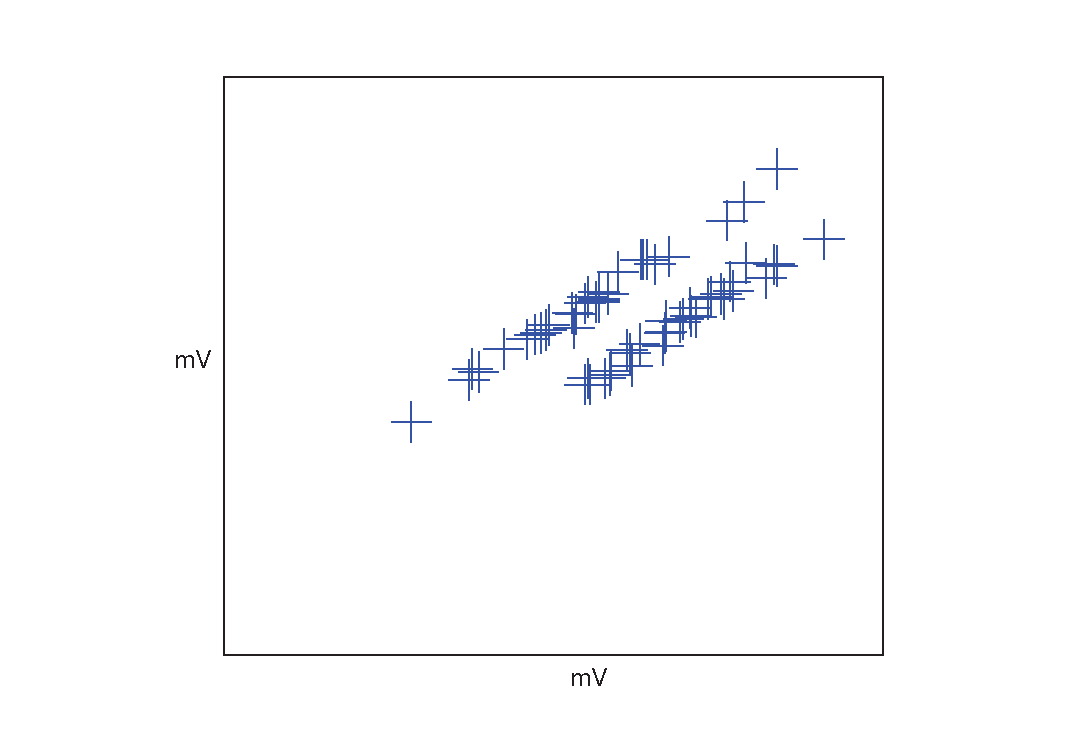
\includegraphics[width=.5\textwidth]{../Figures/PCA_LDA_geometric/PCA_unsupervised_mV2.pdf} 
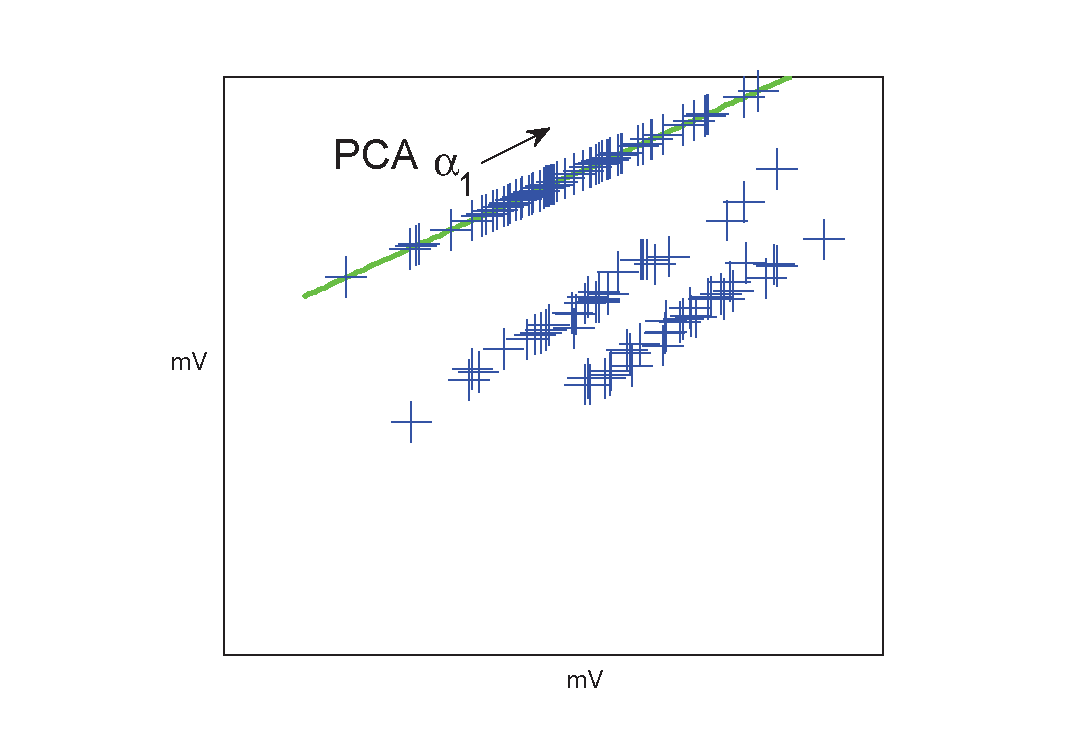
\includegraphics[width=.5\textwidth]{../Figures/PCA_LDA_geometric/PCAprojection_unsupervised_mV2.pdf} 
\caption{PCA: some 2-dimensional data projected into their 1-dimensional principal subspace.}\label{fig:PCAunsupervised}
\end{figure}
The Principal Component Analysis (PCA) is a technique for data dimensionality reduction. The same PCA algorithm can be deduced from two different points of view, a statistical one and a geometrical one. In the former PCA aims to project orthogonally the data onto a lower-dimensional linear space, the so-called \emph{principal subspace}, such that the variance of the projected data is maximized. In the latter, PCA aims to project data onto a lower-dimensional linear space in such a way that the average projection cost, defined as the mean square distance between the data and their projections, is minimized. In the following it is shown how the PCA algorithm is deduced by the statistical definition. The reader interested by the equivalence between the two approaches can refer to \cite[Ch.\ 12]{christopher2006pattern}. An example of 2-dimensional data projected over their 1-dimensional principal subspace is depicted in Fig.~\ref{fig:PCAunsupervised}.\\

Let $(\vLeakVec)_{i=1..\nbTraces}$ be a set of $\traceLength$-dimensional measurements (or observations, or data), i.e. realizations of a $\traceLength$-dimensional zero-mean random vector $\vaLeakVec{}$, and collect them as columns of an $\traceLength \times \nbTraces$ matrix $\measuresMatrix$, so that the empirical covariance matrix of $\vaLeakVec{}$ can be computed as 
\begin{equation}
\covmat = \frac{1}{\nbTraces}\measuresMatrix\measuresMatrix^\intercal \mbox{ .}
\end{equation}

Let us assume for the moment that we have fixed the dimension $\newTraceLength<\traceLength$ of the principal subspace we are looking for. 

\paragraph{Compute the First Principal Component}
Suppose in a first time that $\newTraceLength = 1$, i.e. that we want to represent our data by a unique variable $Y_1 =  \AAlpha_1 \vaLeakVec{}$, i.e. projecting data over a single $ 1 \times\traceLength$ vector $\AAlpha_1$, in such a way the the variance of the obtained data is maximal. The vector $\AAlpha_1$ that provides such a linear combination is called {\em first principal component}. 
To avoid misunderstanding we will call {\em $j$-th principal component} (PC) the projecting vector $\AAlpha_i$, while we will refer to the variable $Y_j = \AAlpha_j \vaLeakVec{}$ as {\em $i$-th Principal Variable (PV)}. 
Realizations of the PVs are given by the measured data projected over the $j$-th PC, for example we have $\nbTraces $ realizations of $Y_1$:
\begin{equation}
y_1[i] = \AAlpha_1 \vLeakVec \mbox{ for } i=1,\dots , \nbTraces \mbox{ .}
\end{equation}

Let us collect these realizations in a vector $\yyy_1 = \AAlpha_1 \measuresMatrix $; the mean of these realizations will be zero as they are linear combinations of zero-mean variables, and the variance turns to be expressible as
\begin{equation}
\frac{1}{\nbTraces}\yyy_1\yyy_1^\intercal = \frac{1}{\nbTraces}\AAlpha_1\measuresMatrix\measuresMatrix^\intercal\AAlpha_1^\intercal = \AAlpha_1\covmat\AAlpha_1^\intercal \mbox{ .}
\end{equation}
To compute $\AAlpha_1$ we have to look for the vector that maximize such a variance.\\

Obviously, we can attend a value for the variance as high as wished, raising the modulo $\|\AAlpha_1\| = \sqrt{\AAlpha_1^T\AAlpha_1}$. In order to let the maximization problem have a solution, we impose a restriction over it: $\AAlpha_1^T\AAlpha_1 = 1$.\\
Let us handle this constrained optimization problem making use of Lagrange multipliers:
\begin{equation}
\Lambda(\AAlpha_1, \lambda) = \AAlpha_1\covmat\AAlpha_1^\intercal - \lambda(\AAlpha_1\AAlpha_1^\intercal-1)
\end{equation}
and let us compute de partial derivative of $\Lambda$ with respect to $\AAlpha_1$
\begin{equation}
\frac{\partial\Lambda}{\partial\AAlpha_1} = 2\covmat\AAlpha_1^\intercal-2\lambda\AAlpha_1^\intercal \mbox{ .}
\end{equation}
Thus, stationary points of $\Lambda$ verify
\begin{equation}\label{eq:eigProblem}
\covmat\AAlpha_1^\intercal = \lambda\AAlpha_1^\intercal \mbox{ ,}
\end{equation}
which implies that $\AAlpha_1^\intercal$ must be an eigenvector of $\covmat$, with $\lambda$ its correspondent eigenvalue. Multiplying both sides of Eq.~(\ref{eq:eigProblem}) by $\AAlpha_1$ on the left, we remark that
\begin{equation}
\AAlpha_1\covmat\AAlpha_1^\intercal = \lambda\AAlpha_1\AAlpha_1^\intercal = \lambda, 
\end{equation}
which means that the variance of the obtained variable $\yyy_1$ equals $\lambda$. For this reason $\AAlpha_1$ must be the leading eigenvector of $\covmat$.

\paragraph{Compute the Second and Following Principal Components}
The PCs following the first one are defined in an incremental fashion by choosing new directions orthogonal to those already considered and such that the sum of the projected variances over each direction is maximal. Explicitly, if we look for two PCs, \ie $\newTraceLength = 2$,  we look for a $2$-dimensional variable $\YYY = \begin{psmallmatrix} \AAlpha_1 \\ \AAlpha_2 \end{psmallmatrix} \vaLeakVec$ such that the trace of its covariance matrix, \ie the sum of variances $\var(Y_1)+\var(Y_2)$, is maximal. It can be shown that the same result would be obtained maximizing the so-called \emph{generalized variance} of $\YYY$, which is defined as the determinant of its covariance matrix, instead of its trace. \\

Let us write, as in previous case, the Lagrangian of the problem
\begin{equation}
\Lambda = \AAlpha_1 \covmat \AAlpha_1^\intercal + \AAlpha_2\covmat \AAlpha_2^\intercal - \lambda_1(\AAlpha_1\AAlpha_1^\intercal -1) - \lambda_2(\AAlpha_2\AAlpha_2^\intercal -1) \mbox{ .}
\end{equation}

Partial derivatives with respect to $\AAlpha_1$ and $\AAlpha_2$ attend zero under the following conditions:
\begin{align}
\covmat  \AAlpha_1^\intercal &= \lambda_1\AAlpha_1^\intercal\\
\covmat  \AAlpha_2^\intercal &= \lambda_2\AAlpha_2^\intercal \mbox{ ,}
\end{align}

which means that $\AAlpha_1^\intercal$ and $\AAlpha_2^\intercal$ must be eigenvectors of $\covmat$ with correspondent eigenvalues given by $\lambda_1$ and $\lambda_2$. Moreover, as before, $\lambda_1$ and $\lambda_2$ equal the variances of variable components $Y_1$ and $Y_2$, and since we want to maximize the sum of such variables we have to choose $\AAlpha_1$ and $\AAlpha_2$ as the two leading vectors of $\covmat$.\\
Let us remark that the covariance between $Y_1$ and $Y_2$ is given by $\AAlpha_1^T\covmat \AAlpha_2$ which equals zero, since $\AAlpha_1^T\AAlpha_2 = 0$, by orthogonality. In particular the principal variables are uncorrelated, which is a remarkable property of the PCA. \\

In the general case of a $\newTraceLength$-dimensional projection space, it can be shown by induction that the PCs would corresponds to the $\newTraceLength$ leading eigenvectors of the covariance matrix $\covmat$.



%----------------------------------------------------------------------------------------
%	SECTION 3
%----------------------------------------------------------------------------------------
\section{Application of PCA in SCAs}\label{sec:PCA_SCA}
\subsection{Original vs Class-Oriented PCA}
\begin{figure}
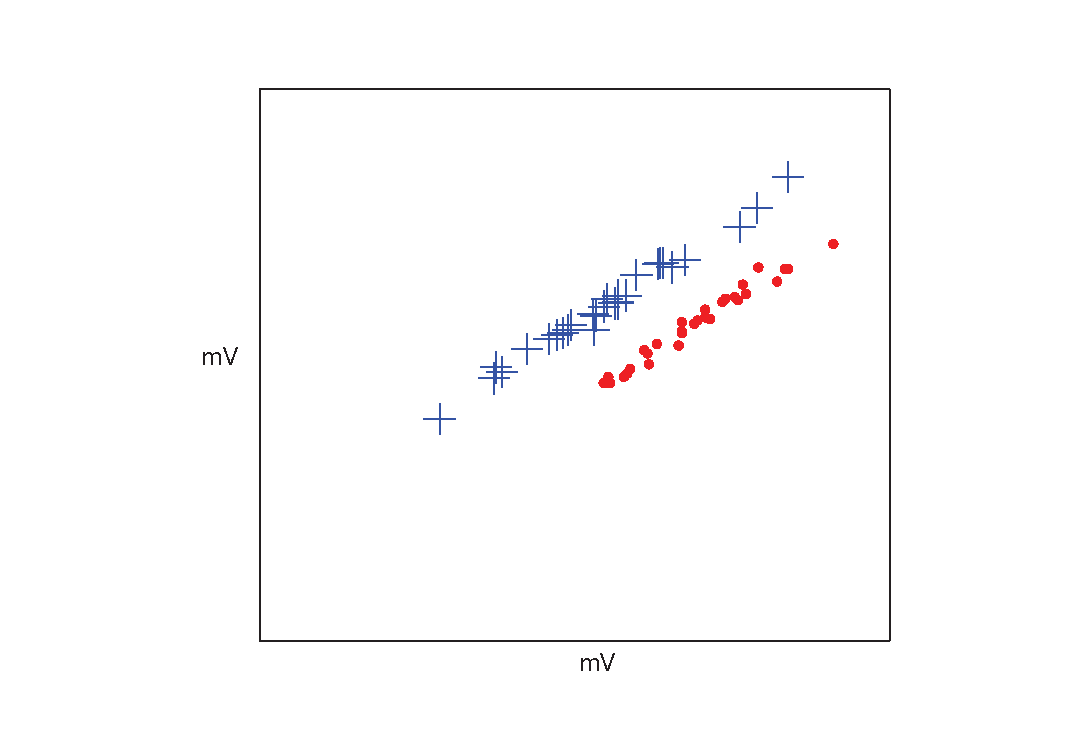
\includegraphics[width=.5\textwidth]{../Figures/PCA_LDA_geometric/dataNoProjection_mV2.pdf} 
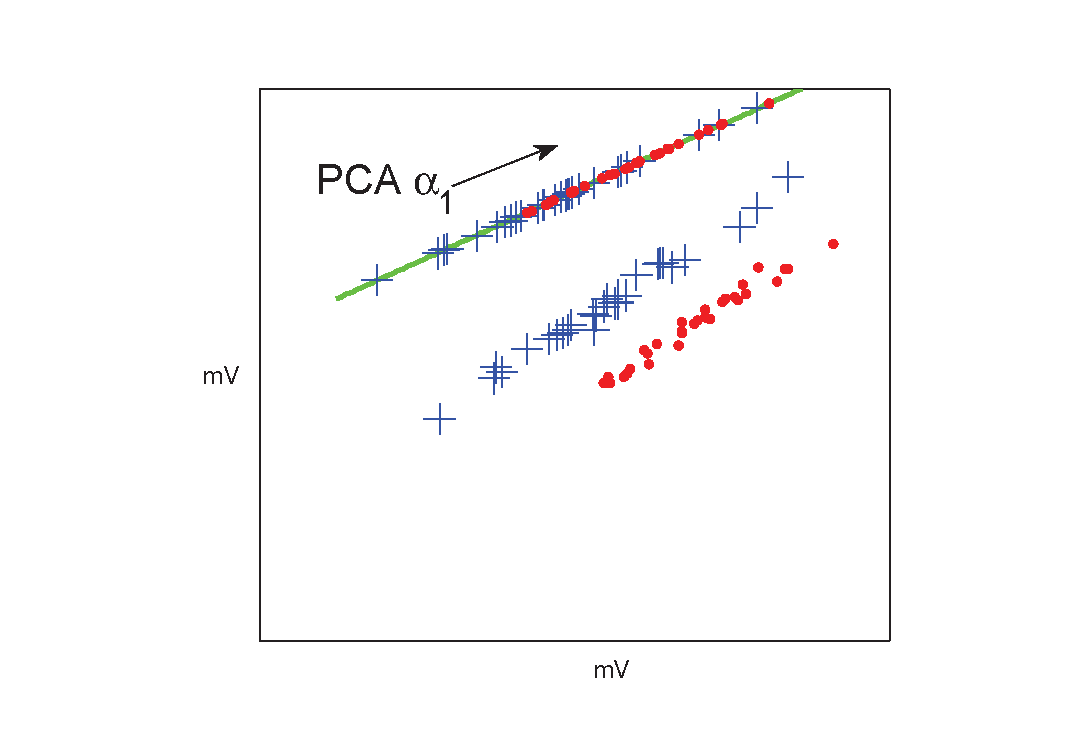
\includegraphics[width=.5\textwidth]{../Figures/PCA_LDA_geometric/PCAprojection_mV2.pdf} 
\caption{PCA: some 2-dimensional data projected into their 1-dimensional principal subspace.}\label{fig:PCAunsupervised}
\end{figure}
The classical version of PCA method is unsupervised.
% in the sense that is does not take into account the information about the value assumed by the target variable during the acquisition of data. 
On the other hand a profiling attacker is provided not only with a set of data $(\vLeakVec)_{i=1..\nbTraces}$, but he can group such traces depending on the target value: this let him obtain a labelled set of traces $(\vLeakVec_i, \sensVar_i)_{i=1..\nbProfilingTraces}$. \\
In this context, and for the sake of distinguishing the target value assumed by the target $\sensRandVar$ in new executions, the idea of the {\em Class-Oriented} PCA is to consider {\em equivalent} all traces belonging to the same class. Modelling traces of a same class as traces showing the same characteristic form plus a random noise, the denoised characteristic form can be estimated by the sample means of the traces in the trace. Supposing that the profiling trace set is balanced, \ie $\nbProfilingTraces = \numClasses \times \nbTraces$ for some $\nbTraces$, the sample means are given by $\mmmXclass = \frac{1}{\nbTraces}\sum_{i\colon \sensVar_i=\sensVar} \vLeakVec_i$. In class-oriented PCA these sample means takes the place of rough data: we collect them as rows in the data matrix $\measuresMatrix$, shift the empirical mean of each component to zero, compute the covariance matrix $\covmat$ et select the leading $\newTraceLength$ eigenvectors of $\covmat$ as optimal projecting directions.\\
In this way we focus the attention on information that discriminate the characteristic forms of classes, \ie target values. 

\subsection{The Choice of the Principal Components}\label{sec:ELV}
The introduction of the PCA method in SCA context (either in its classical or class-oriented version)  has raised some important questions: \textit{how many} principal components and \textit{which ones} are sufficient/necessary to reduce the trace size (and thus the attack processing complexity) without losing important discriminative information?\\

Until 2015, an answer to the questions above was given in \cite{choudary2014efficient}, linked to the concept of {\em explained variance} (or {\em explained global variance}, EGV for short) of a PC $\AAlpha_i$:
\begin{equation}\label{eq:EGV}
\mathrm{EGV}(\AAlpha_i) =  \frac{\lambda_i}{\sum_{k=1}^r\lambda_k} \mbox{ ,}
\end{equation}
where $r$ is the rank of the covariance matrix $\covmat$, and $\lambda_j$ is the eigenvalue associated to the $j$-th PC $\AAlpha_j$. $\mathrm{EGV}(\AAlpha_i)$ is the variance of the data projected over the $i$-th PC (which equals $\lambda_i$) divided by the total variance of the original data (given by the trace of the covariance matrix $\covmat$, \ie by the sum of all its non-zero eigenvalues). By definition of EGV, the sum of all the EGV values is equal to $1$; for this reason this quantity is often multiplied by $100$ and expressed as percentage.
Exploiting the EGV to choose among the PCs consists in fixing a wished {\em cumulative explained variance} $\beta$ and in keeping $\newTraceLength$ different PCs, where $\newTraceLength$ is the minimum integer such that
\begin{equation}
\mbox{EGV}(\AAlpha_1) +\mbox{EGV}(\AAlpha_2) + \dots +\mbox{EGV}(\AAlpha_\newTraceLength) \geq \beta \mbox{ .}
\end{equation}
However, if the attacker has a constraint for the reduced dimension $\newTraceLength$, the EGV notion simply suggests to keep the first $\newTraceLength$ components, taking for granted that the optimal way to chose PCs is in their natural order. This assumption is not always confirmed in SCA context: in some works, researchers have already remarked that the first components sometimes contain more noise than information \cite{Batina2012,specht} and it is worth discarding them. For the sake of providing a first example of this behaviour on publicly accessible traces, we applied a class-oriented PCA on 3000 traces from the DPA contest v4 \cite{DPAcontest}; we focused over a small 1000-dimensional window in which, in complete knowledge about masks and other countermeasures, information about the first Sbox processing leaks (during the first round). In Fig.~\ref{fig:DPAcontest} the first and the sixth PCs are plotted. It may be noticed that the first component indicates that one can attend a high variance by exploiting the regularity of the traces, given by the clock signal, while the sixth one has high coefficients localised in a small time interval, very likely to signalize the instants in which the target sensitive variable leaks.

\begin{figure}
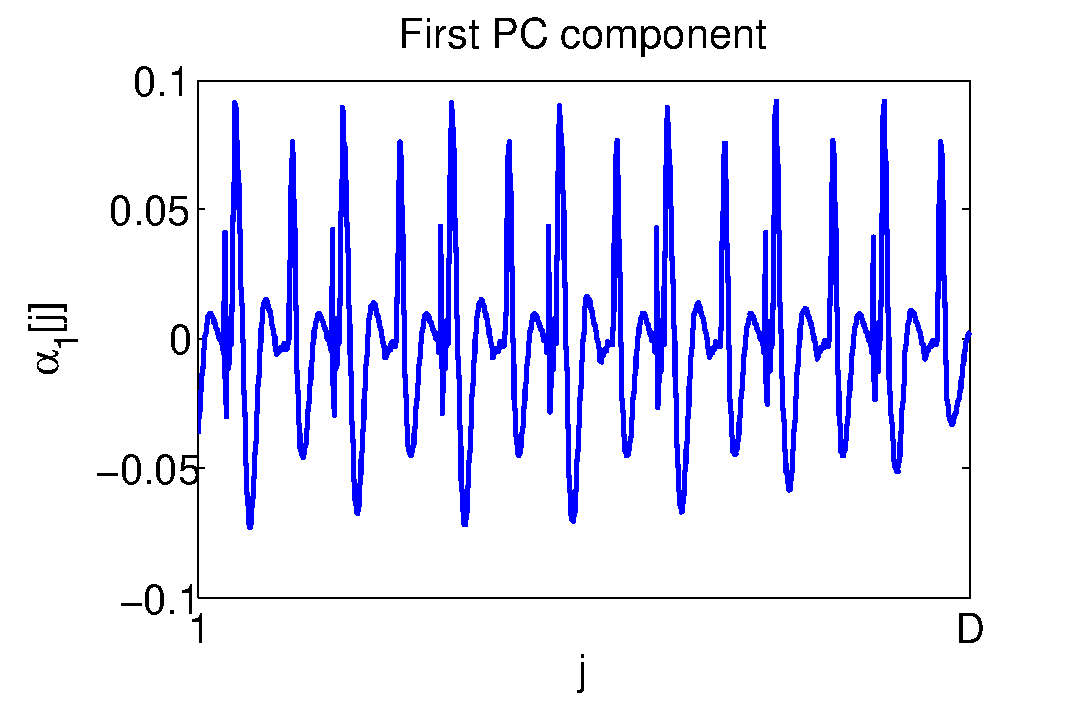
\includegraphics[width=.45\textwidth]{../Figures/CARDIS2015/DPAcontestPC1_new.pdf} 
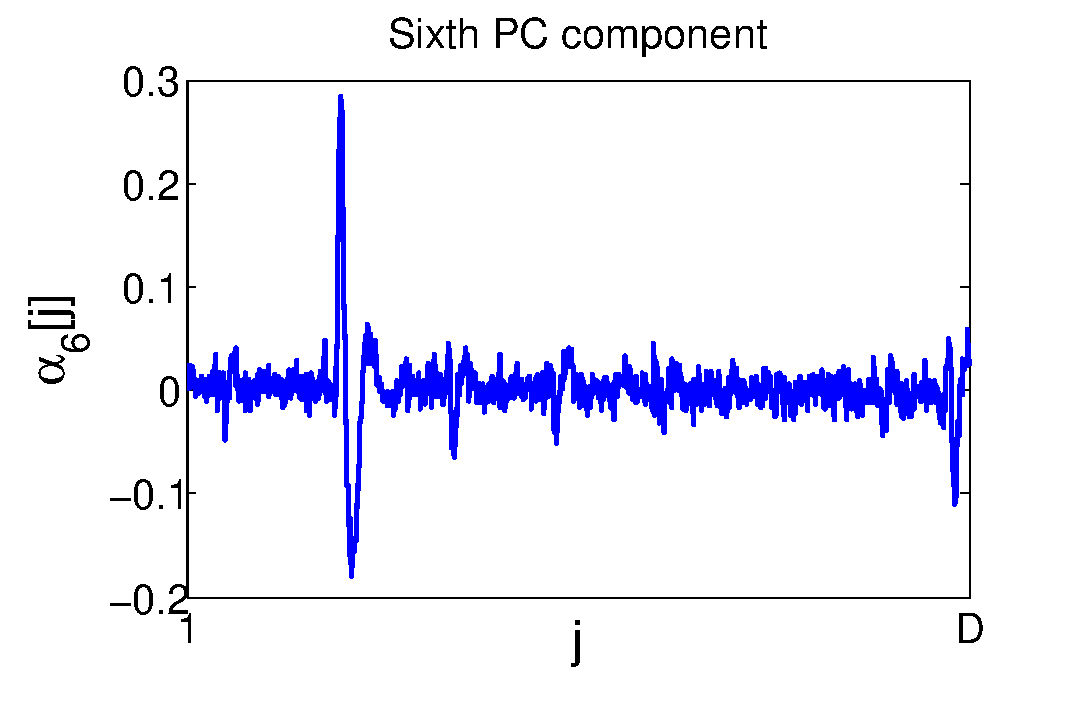
\includegraphics[width=.45\textwidth]{../Figures/CARDIS2015/DPAcontestPC6_new.pdf} 
\caption{First and sixth PCs in DPA contest v4 trace set (between time samples 198001 and 199000)}\label{fig:DPAcontest}
\end{figure}
To the best of our knowledge, a single method adapted to SCA context has been proposed until now to automatically choose PCs \cite{SCAclassProbl} while dealing with the issue raised in Fig.~\ref{fig:DPAcontest}. It is based on the following assumption:
\begin{assumption}\label{assum:local}
The leaking side-channel information is localised in few points of the acquired trace.
\end{assumption}
In the rest of the paper, we conduct our own analyses under Assumption \ref{assum:local} that we think to be reasonable in SCA contexts where the goal of the security developers is to minimize the number of leaking points.
Under this assumption, the authors of \cite{SCAclassProbl} use for side-channel attack purposes the {\em Inverse Participation Ratio} (IPR), a measure widely exploited in Quantum Mechanics domain (see for example \cite{guhr1998random}). They propose to use such a score to evaluate the eigenvectors {\em localization}. It is defined as follows:
\begin{equation}
\mathrm{IPR}(\AAlpha_i) = \sum_{j=1}^\traceLength \AAlpha_i[j]^4 \mbox{ .}
\end{equation}
The authors of \cite{SCAclassProbl} suggest to collect the PCs in decreasing order with respect to the IPR score.\\

The selection methods provided by the evaluation of the EGV and of the IPR are somehow complementary: the former is based only on the eigenvalues associated to the PCs and does not consider the form of the PCs themselves; the latter completely discards the information given by the eigenvalues of the PCs, considering only the distribution of their coefficients. One of the contributions of the present paper is to propose a new selection method, that builds a bridge between the EGV and the IPR approaches. As we will argue, our method, based on the so-called {\em explained local variance}, does not only lead to the construction of a new selection criterion, but also permits  to modify the PCs, choosing individually the coefficients to keep and those to discard. 

\subsection{The Explained Local Variance Selection Method}
The method we develop in this section is based on a compromise between the variance provided by each PC (more precisely its EGV) and the number of time samples necessary to achieve a consistent part of such a variance. To this purpose we  introduce the concept of {\em Explained Local Variance} (ELV).
\begin{figure}
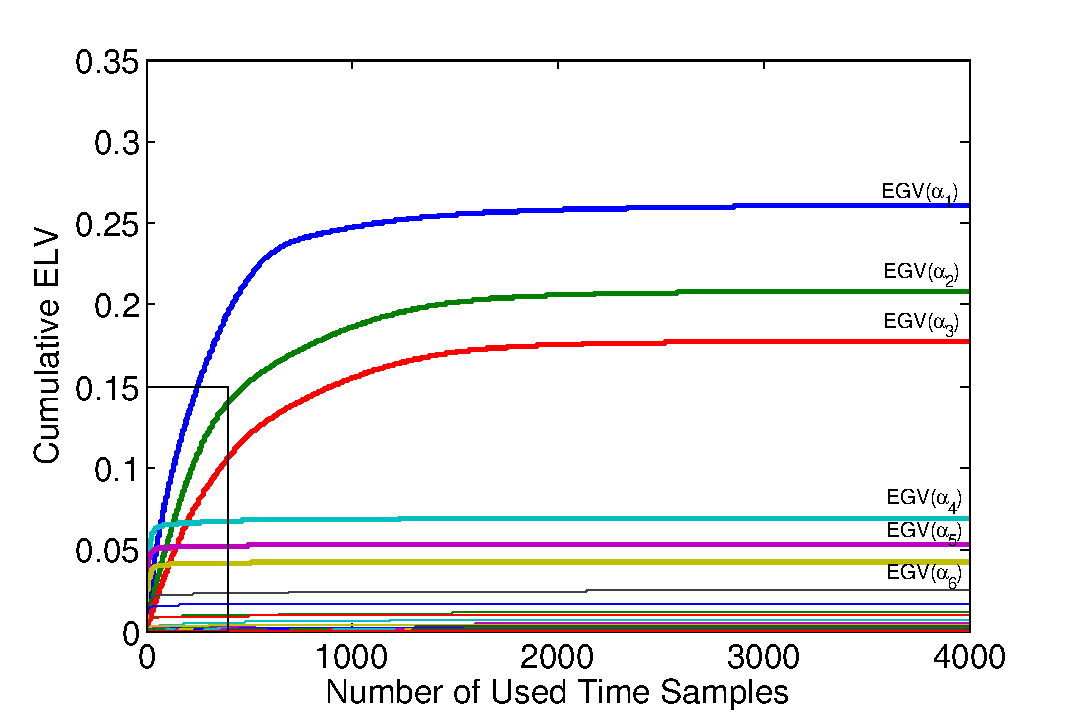
\includegraphics[width=0.5\textwidth]{../Figures/CARDIS2015/cumulativeELVallRectangle.pdf} 
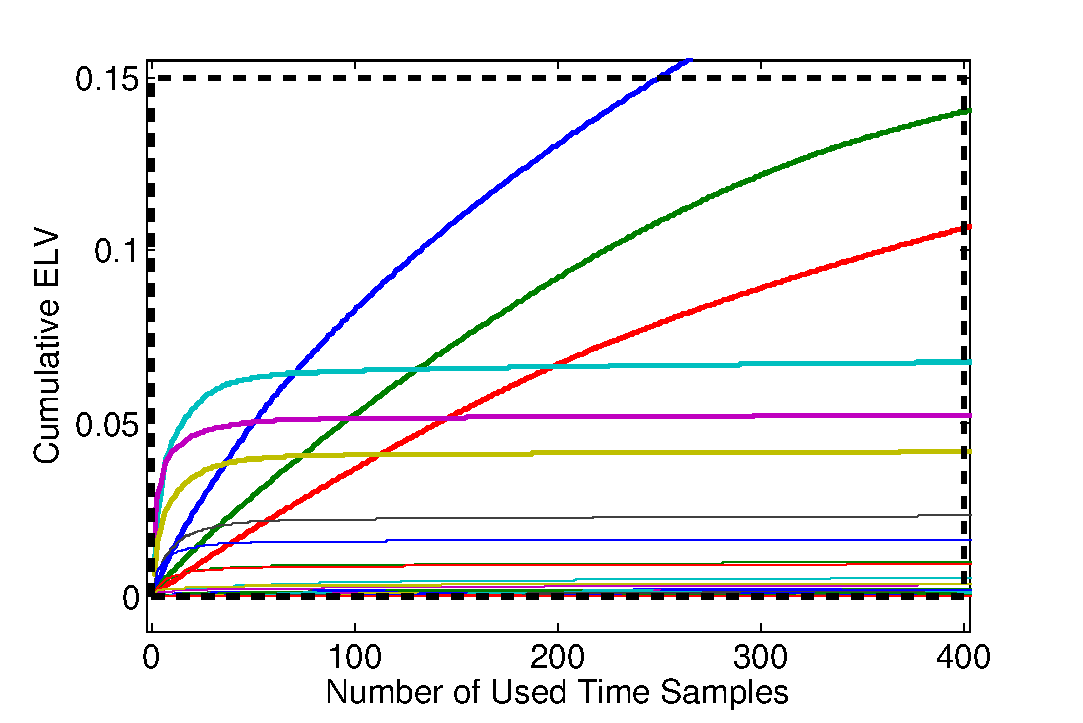
\includegraphics[width=0.5\textwidth]{../Figures/CARDIS2015/cumulativeELVzoomedRectangle.pdf} 
\caption{Cumulative ELV trend of principal components. On the right a zoom of the plot on the left. Data acquisition described in Sec.~\ref{sec:experiments}.}\label{fig:ELVcumulative}
\end{figure}
%
Let us start by giving some intuition behind our new concept. Thinking to the observations ${\vLeakVec}^\intercal$, or to the class-averages ${\mmmX}^\intercal$ in class-oriented PCA case, as realizations of a random variable $\vaLeakVec^\intercal$, we have that $\lambda_i$ is an estimator for the variance of the random variable $\vaLeakVec^\intercal\cdot\AAlpha_i$. Developing, we obtain
\begin{align}\label{eq:ELV}
\lambda_i =& \hat{\var}(\sum_{j=1}^\traceLength \vaLeakVec^\intercal[j]\AAlpha_i[j]) = \sum_{j=1}^\traceLength\sum_{k=1}^\traceLength \hat{\cov}(\vaLeakVec^\intercal[j]\AAlpha_i[j], \vaLeakVec^\intercal[k]\AAlpha_i[k])=\\
=& \sum_{j=1}^\traceLength \AAlpha_i[j]\sum_{k=1}^\traceLength\AAlpha_i[k]\hat{\cov}(\vaLeakVec^\intercal[j], \vaLeakVec^\intercal[k])= \sum_{j=1}^\traceLength \AAlpha_i[j] (\covmat_{j}^\intercal \cdot \AAlpha_i)=  \\
=& \sum_{j=1}^\traceLength \AAlpha_i[j] \lambda_i\AAlpha_i[j]= \sum_{j=1}^\traceLength  \lambda_i \AAlpha_i[j]^2 \label{eq:toJustify}
\end{align}
where $\covmat_{j}^\intercal$ denotes the $j$-th row of $\covmat$ and \eqref{eq:toJustify} is justified by the fact that $\AAlpha_i$ is an eigenvector of $\covmat$, with $\lambda_i$ its corresponding eigenvalue. The result of this computation is quite obvious, since $\parallel \AAlpha_i\parallel=1$, but it evidences the contribution of each time sample in the information held by the PC. This makes us introduce the following definition:
\begin{definition}


The {\em Explained Local Variance} of a PC $\AAlpha_i$ in a sample $j$, is defined by
\begin{equation}
\mathrm{ELV}(\AAlpha_i,j) = \frac{\lambda_i \AAlpha_i[j]^2}{\sum_{k=1}^r\lambda_k} = \mathrm{EGV}(\AAlpha_i) \AAlpha_i[j]^2  \mbox{ .}
\end{equation}
\end{definition}
\begin{figure}
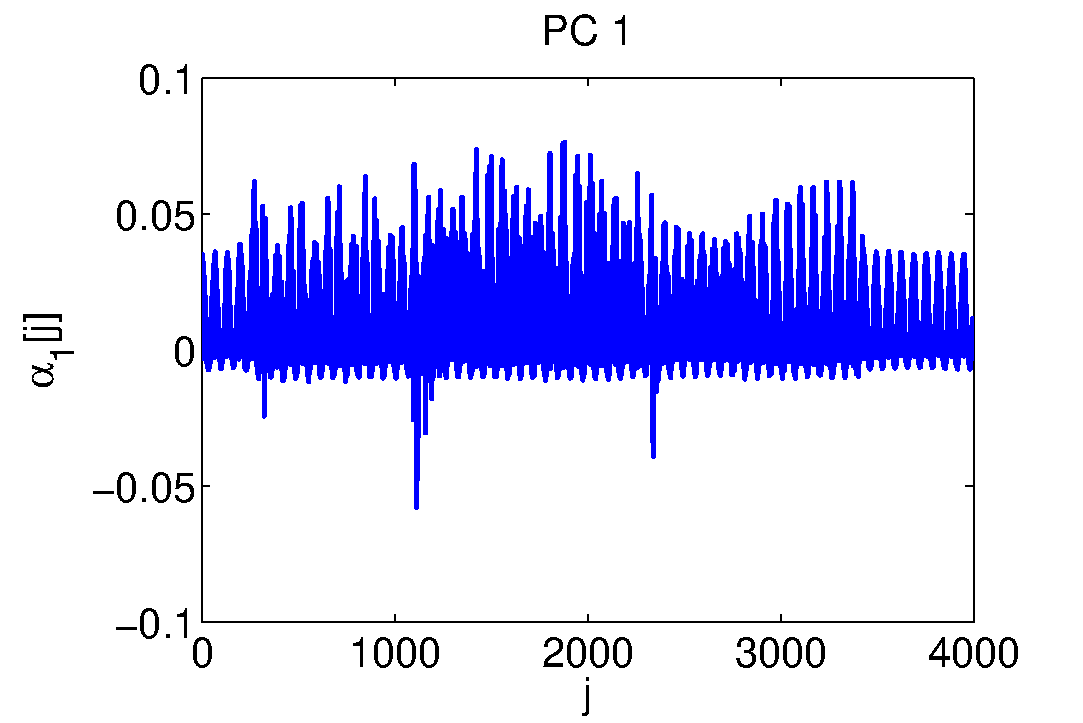
\includegraphics[width=0.31\textwidth]{../Figures/CARDIS2015/PC1.pdf} 
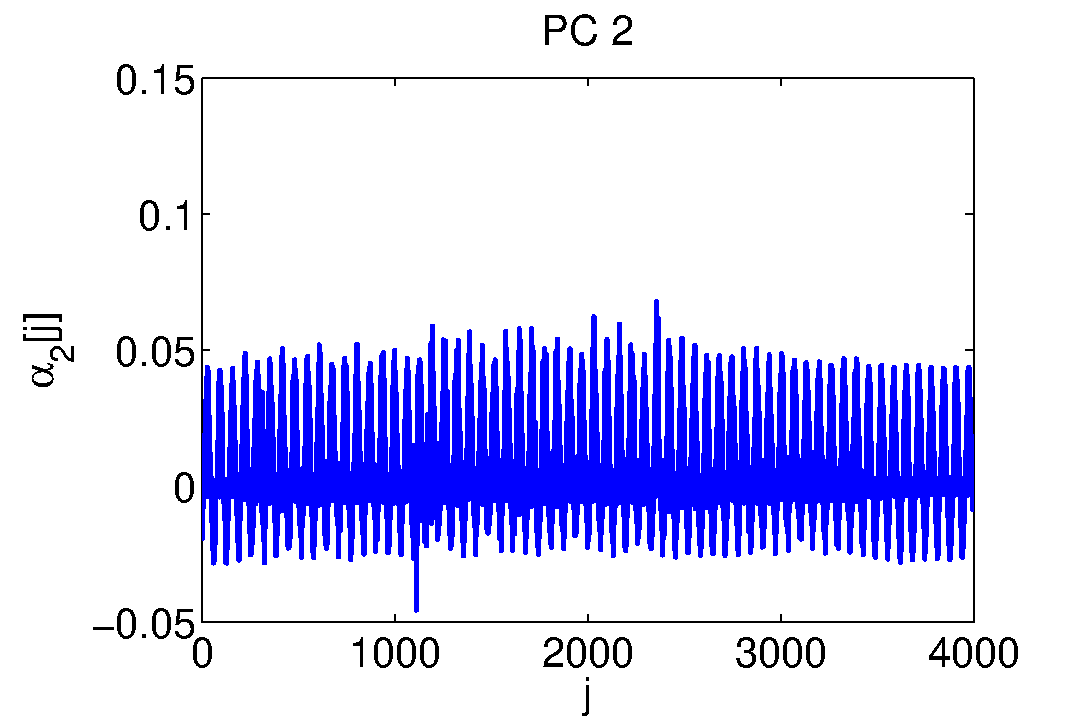
\includegraphics[width=0.31\textwidth]{../Figures/CARDIS2015/PC2.pdf} 
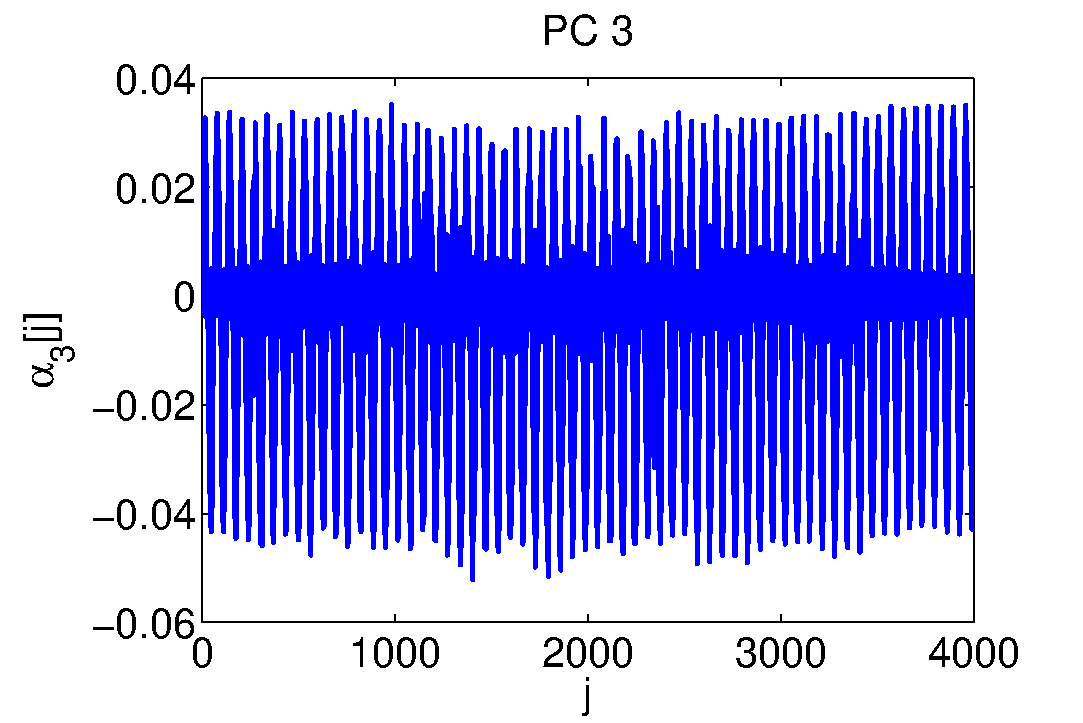
\includegraphics[width=0.31\textwidth]{../Figures/CARDIS2015/PC3.pdf} \\
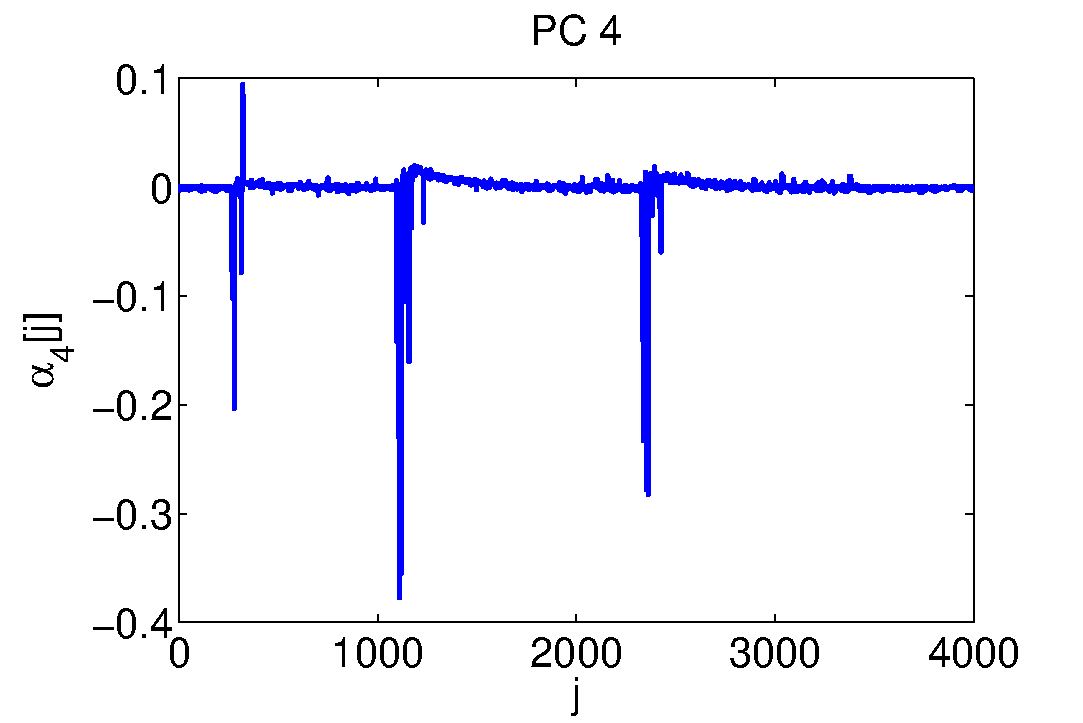
\includegraphics[width=0.31\textwidth]{../Figures/CARDIS2015/PC4.pdf} 
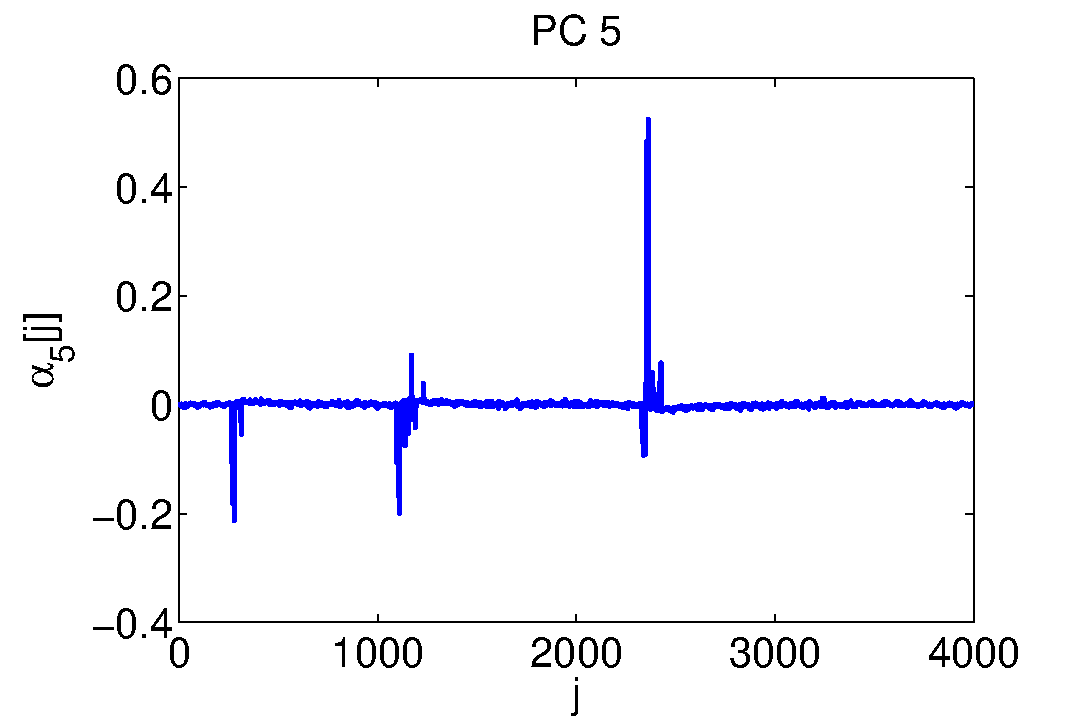
\includegraphics[width=0.31\textwidth]{../Figures/CARDIS2015/PC5.pdf} 
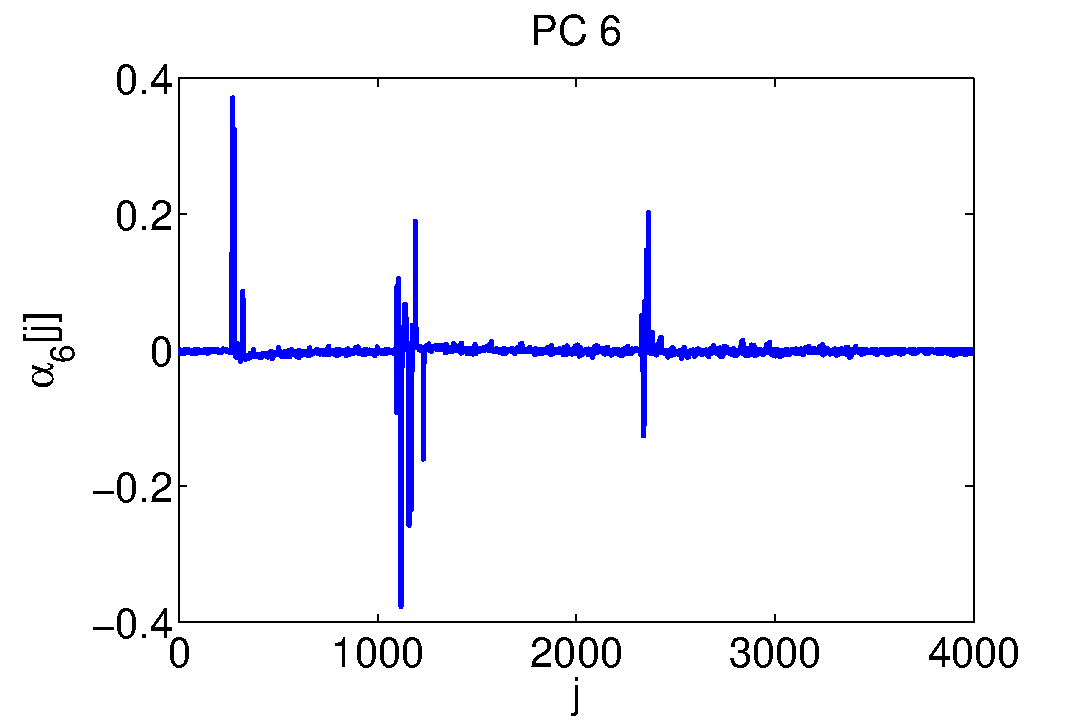
\includegraphics[width=0.31\textwidth]{../Figures/CARDIS2015/PC6.pdf} 
\caption{The first six PCs. Acquisition campaign on an 8-bit AVR Atmega328P (see Sec.~\ref{sec:experiments}).}\label{fig:6components}
\end{figure}
Let $\mathcal{J}=\{j^i_1, j^i_2, \dots, j^i_{\traceLength}\}\subset\{1,2,\dots,\traceLength\}$ be a set of indexes sorted such that $\mathrm{ELV}(\AAlpha_i,j^i_1)\geq \mathrm{ELV}(\AAlpha_i,j^i_2)\geq \dots \geq \mathrm{ELV}(\AAlpha_i,j^i_\traceLength)$.
It may be observed that the sum over all the $\mathrm{ELV}(\AAlpha_i,j)$, for $j\in[1,\dots,\traceLength],$   equals $\mathrm{EGV}(\AAlpha_i)$. If we operate such a sum in a cumulative way following the order provided by the sorted set $\mathcal{J}$, we obtain a complete description of the trend followed by the component $\AAlpha_i$ to achieve its EGV. As we can see in Fig.~\ref{fig:ELVcumulative}, where such cumulative ELVs are represented, the first 3 components are much slower in achieving their final EGV, while the $4^\text{th}$, the $5^\text{th}$ and the $6^\text{th}$ achieve a large part of their final EGVs very quickly ({\em i.e.} by adding the ELV contributions of much less time samples). For instance, for $i=4$, the sum of the $\mathrm{ELV}(\AAlpha_4, j^4_k)$, with $k\in[1,\dots,30]$, almost equals $\mathrm{EGV}(\AAlpha_4)$, whereas the same sum for $i=1$ only achieves about the 15\% of $\mathrm{EGV}(\AAlpha_1)$. Actually, the EGV of the $4^\text{th}$, the $5^\text{th}$ and the $6^\text{th}$ component only essentially depends on a very few time samples. This observation, combined with Assumption \ref{assum:local}, suggests that they are more suitable for SCA than the three first ones. To validate this statement, it suffices to look at the form of such components (Fig.~\ref{fig:6components}): the leading ones are strongly influenced by the clock, while the latest ones are well localised over the leaking points.\\

Operating a selection of components {\em via} ELV, in analogy with the EGV, requires to fix the reduced space dimension $\newTraceLength$, or a threshold $\beta$ for the cumulative ELV. In the first case, the maximal ELVs of each PC are compared, and the $\newTraceLength$ components achieving the highest values of such ELVs are chosen. In the second case, all pairs (PC, time sample) are sorted in decreasing order with respect to their ELV, and summed until the threshold $\beta$ is achieved. Then only PCs contributing in this sum are selected. \\

We remark that the ELV is a score associated not only to the whole components, but to each of their coefficients. This interesting property can be exploited to further remove, within a selected PC, the non-significant points, {\em i.e.} those with a low ELV. In practice this is done by setting these points to zero. That is a natural way to exploit the ELV score in order to operate a kind of {\em denoising} for the reduced data, making them only depend  on the significant time samples. In Sec.~\ref{sec:experiments} (scenario 4) we test the performances of an attack varying the number of time samples involved in the computation of the reduced data, and showing that such a denoising processing might impact significantly. 



%----------------------------------------------------------------------------------------
%	SECTION 4
%----------------------------------------------------------------------------------------

\section{Linear Discriminant Analysis}\label{sec:LDA}

\subsubsection{Fisher's Linear Discriminant and Terminology Remark}
Fisher's Linear Discriminant \cite{Fukunaga} is another statistical tool for dimensionality reduction, which is commonly used as a preliminary step before classification. Indeed it seeks for linear combinations of data that characterize or separate two or more classes, not only spreading class centroids as much as possible, like the class-oriented PCA does, but also minimizing the so-called {\em intra-class variance}, i.e. the variance shown by data belonging to the same class. The terms Fisher's Linear Discriminant and Linear Discriminant Analysis (LDA) are often used interchangeably, and in particular in SCA literature the Fisher's Linear Discriminant is almost always referred to as LDA, \eg \cite{lessIsMore,Standaert2008}. As we anticipated in Chapter~\ref{ChapterIntroML} - Example~\ref{example:LDA}, his widely-accepted abuse is due to the fact that under the assumptions leading to the LDA classification tools (\ie Gaussian class-conditional densities, sharing a common covariance matrix), the solution provided by the Fisher's Linear Discriminant (that does not require such assumptions) is the same as the solution provided by the LDA. From now on we will use the more common terminology LDA to refer to Fisher's Linear Discriminant. \\

\subsubsection{Description.} Applying LDA consists in maximizing the so-called {\em Rayleigh quotient}:
 \begin{equation}\label{eq:LDA}
 \AAlpha_1=\mathrm{argmax}_{\AAlpha} \frac{\AAlpha^\intercal \SB \AAlpha}{\AAlpha^\intercal \SW \AAlpha} \mbox{ ,}
 \end{equation}
where $\SB$ is the {\em between-class scatter matrix} already defined in \eqref{eq:SB} and $\SW$ is called 
{\em within-class} (or intra-class) {\em scatter matrix}:

\begin{equation}
\SW = \sum_{\sensVar\in\sensVarSet}\sum_{i=1}^{\nbProfilingTraces}(\vLeakVec_i-\mmmXclass)(\vLeakVec_i-\mmmXclass)^\intercal \mbox{.}
\end{equation}


\begin{remark}
Let $\covmat$ be the the global covariance matrix of data, also called {\em total scatter matrix}, defined in \eqref{eq:covmat}; we have the following relationship between $\SW,\SB$ and $\covmat$:
\begin{equation}
\covmat = \frac{1}{\nbProfilingTraces}(\SW + \SB) \mbox{ .}
\end{equation}
\end{remark}

It can be shown that the vector $\AAlpha_1$ which maximizes \eqref{eq:LDA} must satisfy $\SB\AAlpha_1 = \lambda \SW \AAlpha_1$, for a constant $\lambda$, \textit{i.e.} has to be an eigenvector of $\SW^{-1} \SB$. Moreover, for any eigenvector $\AAlpha$ of $\SW^{-1}\SB$, with associated eigenvalue $\lambda$, the Rayleigh quotient equals such a $\lambda$:
\begin{equation}\label{eq:lambdas}
\frac{\AAlpha^\intercal \SB \AAlpha}{\AAlpha^\intercal \SW \AAlpha} = \lambda \mbox{ .}
\end{equation}
Then, among all eigenvectors of $\SW^{-1} \SB$, $\AAlpha_1$ must be the leading one.\\

The computation of the eigenvectors of $\SW^{-1} \SB$ is known under the name of {\em generalized eigenvector problem}. The difficulty here comes from the fact that $\SW^{-1} \SB$ is not guaranteed to be symmetric. Due to this non-symmetry,  $\AAlpha_1$ and the others eigenvectors do not form an orthonormal basis for $\mathbb{R}^\traceLength$, but they are anyway useful for classifications scopes, as in SCA. Let us refer to them as {\em Linear Discriminant Components} (LDCs for short); as for PCs we consider them sorted in decreasing order with respect to their associated eigenvalue, which gives a score for their informativeness, see \eqref{eq:lambdas}. Analogously to the PCA, the LDA provides a natural dimensionality reduction: one can project the data over the $\newTraceLength$ first LDCs. As for PCA, this choice might not be optimal when applying this reduction to side-channel traces. For the sake of comparison, we tested all the selection methods proposed for the PCA (EGV, IPR and ELV) in association to the LDA as well.\\

In the following subsection we will present a well-known problem that affects the LDA in many practical contexts, and describe four methods that circumvent such a problem, with the intention to test them over side-channel data.


\subsection{The Small Sample Size Problem}\label{sec:SSS}
In the special case in which the matrix $\SB$ is invertible, the generalized eigenvalue problem is convertible in a regular one, as in \cite{Standaert2008}. On the contrary, when $\SB$ is singular, the simultaneous diagonalization is suggested to solve such a problem \cite{Fukunaga}. In this case one can take advantage by the singularity of $\SB$ to apply the computational trick proposed by Archambeau et al., see Sec.~(\ref{sec:PCA_classes}), since at most $r = \mathrm{rank}(\SB)$ eigenvectors can be found.\\

If the singularity of $\SB$ does not affect the LDA dimensionality reduction, we cannot say the same about the singularity of $\SW$:  SCA and Pattern Recognition literatures point out the same drawback of the LDA, known as the {\em Small Sample Size problem} (SSS for short). It occurs when the total number of acquisitions $\nbProfilingTraces$ is less than or equal to the size $\traceLength$ of them.\footnote{It can happen for example when attacking an RSA implementation, where the acquisitions are often huge (of the order of 1,000,000 points) and the number of measurements may be small when the SNR is good, implying that a good GE can be achieved with a small $N$.} The direct consequence of this problem is the singularity of $\SW$ and the non-applicability of the LDA. \\

If the LDA has been introduced relatively lately in the SCA literature, the Pattern Recognition community looks for a solution to the SSS problem at least since the early nineties. We browsed some of the proposed solutions and chose some of them to introduce, in order to test them over side channel traces.

\subsubsection{Fisherface Method}
The most popular among the solutions to SSS is the so-called {\em Fisherface} method\footnote{The name is due to the fact that it was proposed and tested for face recognition scopes.} \cite{eigenfaces}. It simply relies on the combination between PCA and LDA: a standard PCA dimensionality reduction is performed to data, making them pass from dimension $\traceLength$ to dimension $\nbProfilingTraces-\nbClasses$, which is the general maximal rank for $\SW$. In this reduced space, $\SW$ is very likely to be invertible and the LDA therefore applies.

\subsubsection{$\SW$ Null Space Method}
It has been introduced by Chen et al. in \cite{Chen2000} and exploits an important result of Liu et al. \cite{liu1992generalized} who showed that Fisher's criterion \eqref{eq:LDA} is equivalent to:
 \begin{equation}
 \AAlpha_1=\mathrm{argmax}_{\AAlpha} \frac{\AAlpha^\intercal \SB \AAlpha}{\AAlpha^\intercal \SW \AAlpha + \AAlpha^\intercal \SB \AAlpha} \mbox{ .}
 \end{equation}
The authors of \cite{Chen2000} point out that such a formula is upper-bounded by 1, and that it achieves its maximal value, \textit{i.e.} 1, if and only if  $\AAlpha$ is in the null space of $\SW$. Thus they propose to first project data onto the null space of $\SW$ and then to perform a PCA, \textit{i.e.} to select as LDCs the first $\nbClasses - 1$ eigenvectors of the between-class scatter matrix of data into this new space. More precisely, let $Q = [\vvv_1, \dots, \vvv_{\traceLength - \mathrm{rank}(\SW)}]$ be the matrix of vectors that span the null space of $\SW$. \cite{Chen2000} proposes to transform the data $\vLeakVec$ into $\vLeakVec^\prime = QQ^\intercal\vLeakVec$. Such a transformation maintains the original dimension $\traceLength$ of the data, but let the new within-class matrix $\SW' = QQ^\intercal\SW QQ^\intercal$ be the null $\traceLength \times \traceLength$ matrix. Afterwards, the method looks for the eigenvectors of the new between-class matrix $\SB' = QQ^\intercal\SB QQ^\intercal$. Let $U$ be the matrix containing its first $\nbClasses - 1$ eigenvectors: the LDCs obtained via the $\SW$ null space method are the columns of $QQ^\intercal U$.

\subsubsection{Direct LDA}
As the previous, this method, introduced in \cite{Yu01adirect}, privileges the low-ranked eigenvectors of $\SW$, but proposes to firstly project the data onto the rank space of $\SB$, arguing the fact that vectors of the null space of $\SB$ do not provide any between-class separation of data. Let $D_B=V^\intercal\SB V$ be the diagonalization of $\SB$, and let $V^\star$ be the matrix of the eigenvectors of $\SB$ that are not in its null space, \textit{i.e.} whose eigenvalues are different from zero. Let also $D_B^\star$ denotes the matrix ${V^\star}^\intercal\SB V^\star$; transforming the data $\vLeakVec$ into ${D_B^\star}^{1/2}{V^\star}^\intercal\vLeakVec$ makes the between-class variance to be equal to   the $(\nbClasses - 1) \times (\nbClasses- 1)$ identity matrix. After this transformation the within-class variance assumes the form $\SW' = {D_B^\star}^{1/2}{V^\star}^\intercal\SW ' V^\star {D_B^\star}^{1/2}$. After storing the $\newTraceLength$ lowest-rank eigenvectors in a matrix $U^\star$, the LDCs obtained via the Direct LDA method are the columns of $V^\star{D_B^\star}^{1/2}{U^\star}^\intercal$. 


\subsubsection{$\ST$ Spanned Space Method}
The last variant of LDA that we consider has been proposed in \cite{huang} and is actually a variant of the Direct LDA: instead of removing the null space of $\SB$ as first step, this method removes the null space of $\ST = \SB + \SW$. Then, denoting $\SW'$ the within-class matrix in the reduced space, the reduced data are projected onto its null space, i.e. are multiplied by the matrix storing by columns the eigenvectors of $\SW'$ associated to the null eigenvector, thus reduced again. A final optional step consists in verifying whether  the between-class matrix presents a non-trivial null-space after the last projection and, in this case, in effectuating a further projection removing it.

\begin{remark}
Let us remark that, from a computational complexity point of view (see \cite{huang} for a deeper discussion), the least time-consuming procedure among the four proposed is the Direct LDA, followed by the Fisherface and the $\ST$ Spanned Space Method, that have a similar complexity. The $\SW$ Null Space Method is in general much more expensive, because the task of removing the $\SW$ null space requires the actual computation of the $(\traceLength\times \traceLength)$-dimensional matrix $\SW$, {\em i.e.} the computational trick proposed by Archambeau et al. \cite{TAprincipal}, see Sec.~\ref{sec:PCA_classes} is not applicable. On the contrary, the other three methods take advantage of such a procedure, reducing drastically their complexity.
\end{remark}



%----------------------------------------------------------------------------------------
%	SECTION 6
%----------------------------------------------------------------------------------------


\section{Experimental Results}\label{sec:experiments}

In this section we compare the different extractors (\ie functions applying a data dimensionality reduction, see Sec.~\ref{sec:extractors}) provided by the PCA and the LDA in association with the different techniques  of components selection. Defining an universal criterion to compare the different extractors would not make sense since the latter one should encompass a lot of parameters, sometimes opposite, that vary according to the context (amount of noise, specificity of the information leakage, nature of the side channel, etc.). For this reason we choose to split our comparisons into four scenarios. Each scenario has a single varying parameter that, depending on the attacker context, may wish to be minimized. Hereafter the definition of the four scenario. In the following only results of the two first is reported, the interested reader might refer to Appendix\ref{Appendix_scenario3_4_cardis2015} for results of in the two other scenarios.  
\begin{itemize}
\item[Scenario 1] varying parameter: number of attack traces $\nbAttackTraces$, 
\item[Scenario 2] varying parameter: number of profiling traces $\nbProfilingTraces$, 
\item[Scenario 3] varying parameter: number of projecting components selected $\newTraceLength$,
\item[Scenario 4] varying parameter: number of original time samples implied into the trace preprocessing computation $\numPoI$ .
\end{itemize}
 
For scenarios in which $\nbProfilingTraces$ is fixed, the value of $\nbProfilingTraces$ is chosen high enough to avoid the SSS problem, and the extensions of LDA presented in Sec.~\ref{sec:SSS} are not evaluated.
 This choice of $\nbProfilingTraces$ will imply that the LDA is always performed in a favourable situation, which makes expect the LDA to be particularly efficient for these experiments. Consequentely, for the scenarios in which $\nbProfilingTraces$ is high, our goal is to study whether the PCA can be made almost as efficient as the LDA thanks to the component selection methods discussed in Sec.~\ref{sec:ELV}. 



\subsubsection{The testing adversary.}  
Our testing adversary attacks an 8-bit AVR microprocessor Atmega328P and acquires power-consumption traces via the ChipWhisperer platform \cite{o2014chipwhisperer}.\footnote{This choice has been done to allow for reproducibility of the experiments.} The target device stores a secret 128-bit key and performs the first steps of an AES: the loading of 16 bytes of the plaintext, the AddRoundKey step and the AES Sbox. It has been programmed twice: two different keys are stored in the device memory during the acquisition of the profiling and of the attack traces, to simulate the situation of two identical devices storing a different secret. The size $\traceLength$ of the traces equals $3996$. The sensitive target  variable is the output of the first Sbox processing, but, since the key is fixed also during the profiling phase, and both Xor and Sbox operations are bijective, we expect to detect three interesting regions (as those high-lighted by PCs 4, 5 and 6, in Fig.~\ref{fig:6components}): the reading of the first byte of the plaintext, the first AddRoundKey and the first Sbox. We consider an {\em identity classification} leaking function (i.e. we make minimal assumption on the leakage function), which implies that the 256 possible values of the Sbox output yields to 256 classes. For each class we assume that the adversary acquires the same number $\nbTraces$ of traces, \textit{i.e.} $\nbProfilingTraces =\nbTraces\times 256$. After the application of the extractor $\extract$, the trace size is reduced to $\newTraceLength$. Then the attacker performs a Template Attack (see Sec.~\ref{sec:TA}, using $\newTraceLength$-variate Gaussian templates.


\begin{figure}[t]
\subfigure[]{\label{fig:1.1}
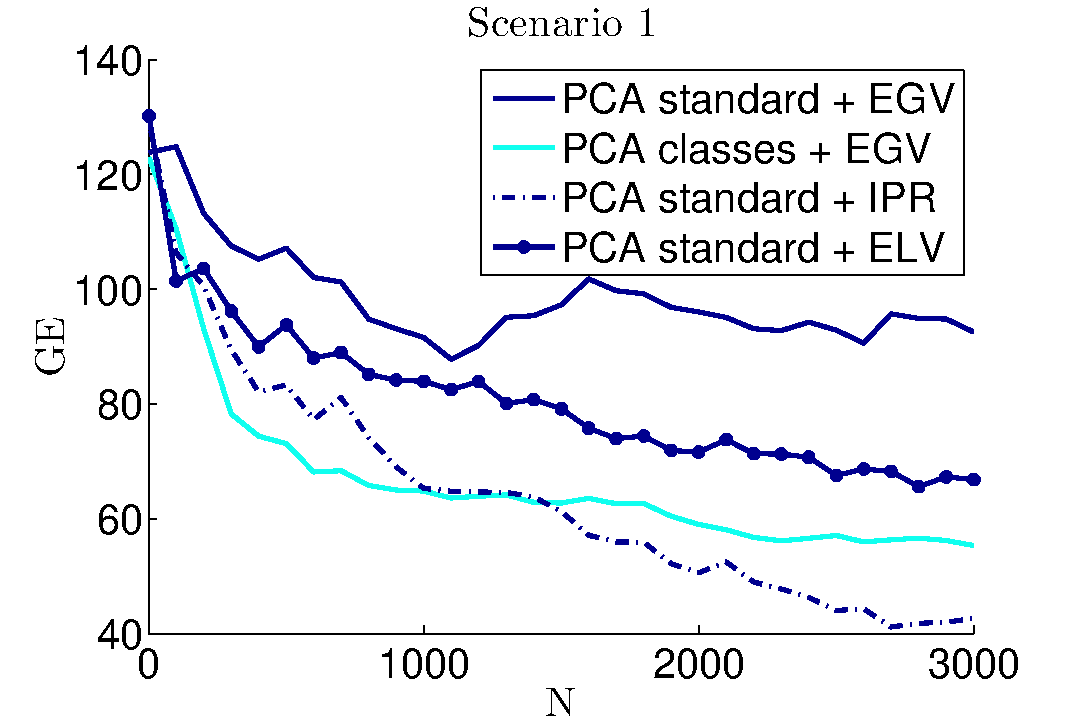
\includegraphics[width=0.5\textwidth]{../Figures/CARDIS2015//Criterion1.pdf}}
\subfigure[]{\label{fig:1.2}
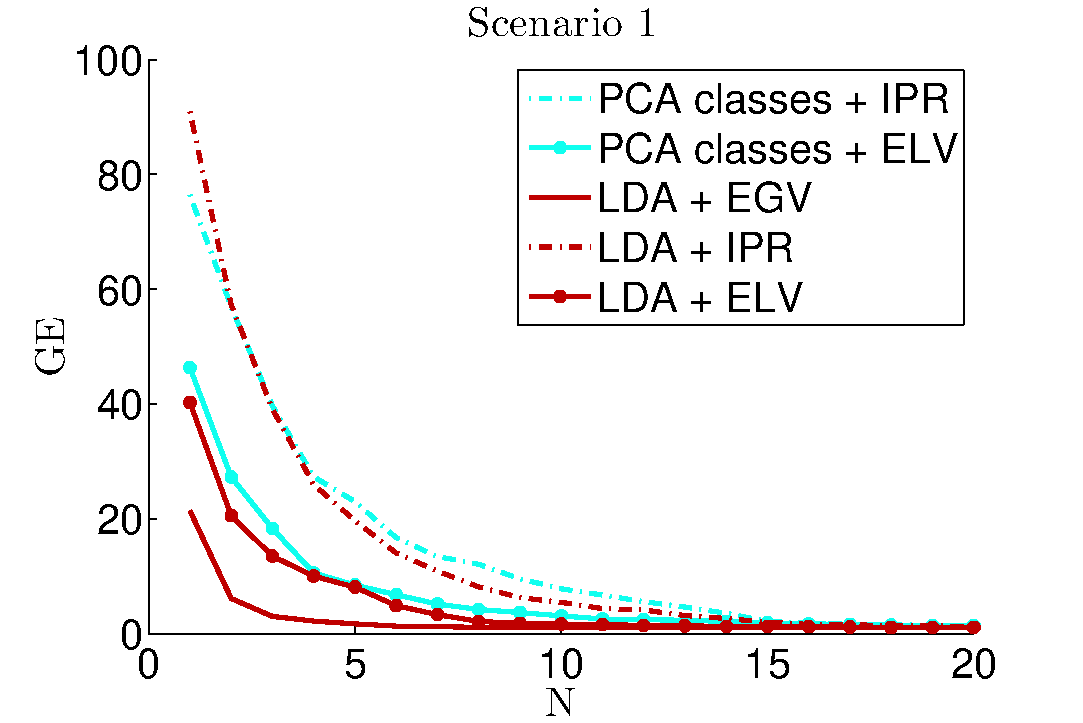
\includegraphics[width=0.5\textwidth]{../Figures/CARDIS2015//Criterion1Good.pdf}}
\caption[Guessing Entropy as function of the number of attack traces]{Guessing Entropy as function of the number of attack traces for different extraction methods. All Guessing Entropies are estimated as the average rank of the right key over 100 independent experiments.}\label{fig:scenario1}
\end{figure}
\subsubsection{Scenario 1.}
To analyse the dependence between the extraction methods presented in Sections~\ref{sec:PCA} and \ref{sec:LDA} and the number of attack traces $\nbAttackTraces$ needed to achieve a given GE, we fixed the other parameters as follows: $\nbTraces=50$ ($\nbProfilingTraces=50\times 256$), $\newTraceLength = 3$ and $\numPoI = 3996$ (all points are allowed to participate in the building of the PCs and of the LDCs). The experimental results, depicted in Fig.~\ref{fig:scenario1}\subref{fig:1.1}-\subref{fig:1.2}, show that the PCA standard method has very bad performances in SCA, while the LDA outperforms the others. Concerning the class-oriented PCA, we observe that its performance is close to that of LDA when combined with the selection methods ELV (which performs best) or IPR.  



\subsubsection{Scenario 2.}
%\begin{figure}
%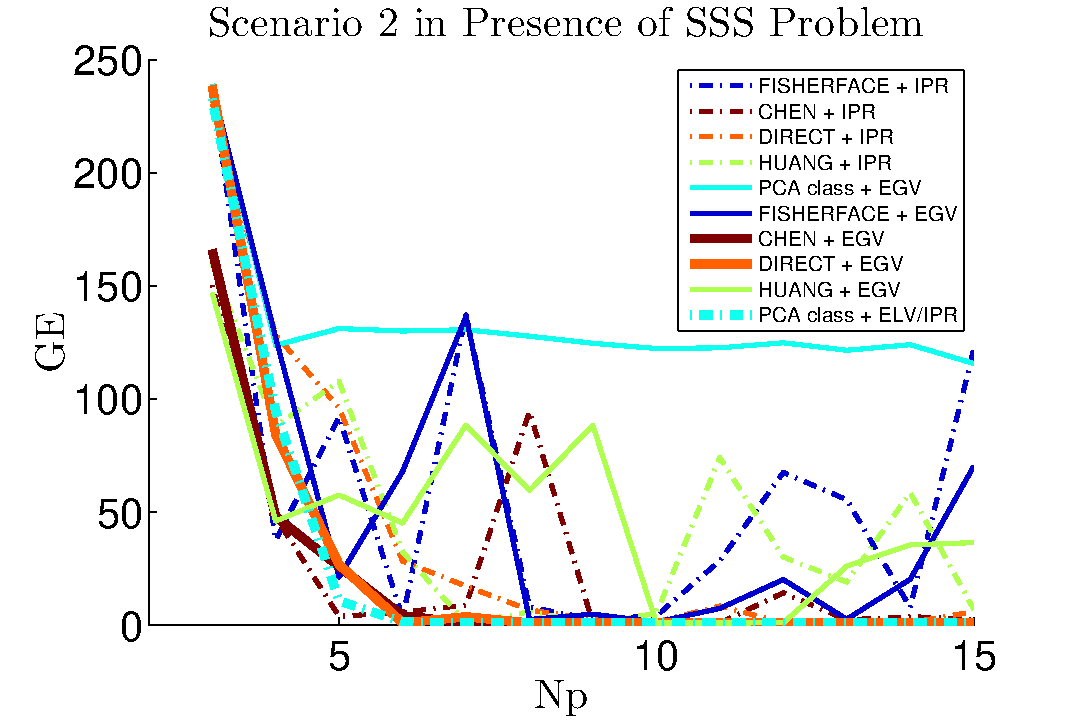
\includegraphics[width=0.5\textwidth]{figures/Criterion2SSS.pdf}
%\includegraphics[width=0.5\textwidth]{figures/Criterion2notSSS.pdf} 
%\caption{Guessing Entropy as function of the number of profiling traces per class, for different extraction methods: on the left the LDA is substituted by its extensions to handle the SSS problem.}\label{fig:2}
%\end{figure}
Now we test the behaviour of the extraction methods as function of the number $N_z$ of available profiling traces per class. The number of components $\newTraceLength$ is still fixed to 3, $\numPoI=3996$ again and the number of attack traces is $\nbAttackTraces=100$. This scenario has to be divided into two parts: if $N_z\leq 15$, then $\nbProfilingTraces<\traceLength$ and the SSS problem occurs. Thus, in this case we test the four extensions of LDA presented in Sec.~\ref{sec:SSS}, associated to either the standard selection, to which we abusively refer as EGV,%\footnote{It consists in keeping the $\newTraceLength$ first LDCs, except for the Direct LDA, which asks to keep the last LDCs.}
\footnote{It consists in keeping the $\newTraceLength$ first LDCs (the $C$ last for the Direct LDA)}
or to the IPR selection.  We compare them to the class-oriented PCA associated to EGV, IPR or ELV. The ELV selection is not performed for the techniques extending LDA, since for some of them the projecting LDCs are not associated to some eigenvalues in a meaningful way. On the contrary, if $\nbTraces \geq 16$ there is no need to approximate the LDA technique, so the classical one is performed. Results for this scenario are shown in Fig.~\ref{fig:scenario2}. It may be noticed that the combinations class-oriented PCA + ELV/IPR select exactly the same components, for our data, see Fig.~\ref{fig:pcaclass} and do not suffer from the lack of profiling traces. They are slightly outperformed by the $\SW$ Null Space method associated with the EGV, see Fig.\ref{fig:swnullspace}. The Direct LDA (Fig.~\ref{fig:direct}) method also provides a good alternative, while the other tested methods do not show a stable behaviour. The results in absence of the SSS problem (Fig.\ref{fig:notSSS}) confirm that the standard PCA is not adapted to SCA, even when provided with more profiling traces. It also shows that among class-oriented PCA and LDA, the class-oriented PCA converges faster.



\begin{figure}
\subfigure[]{\label{fig:fisherface}
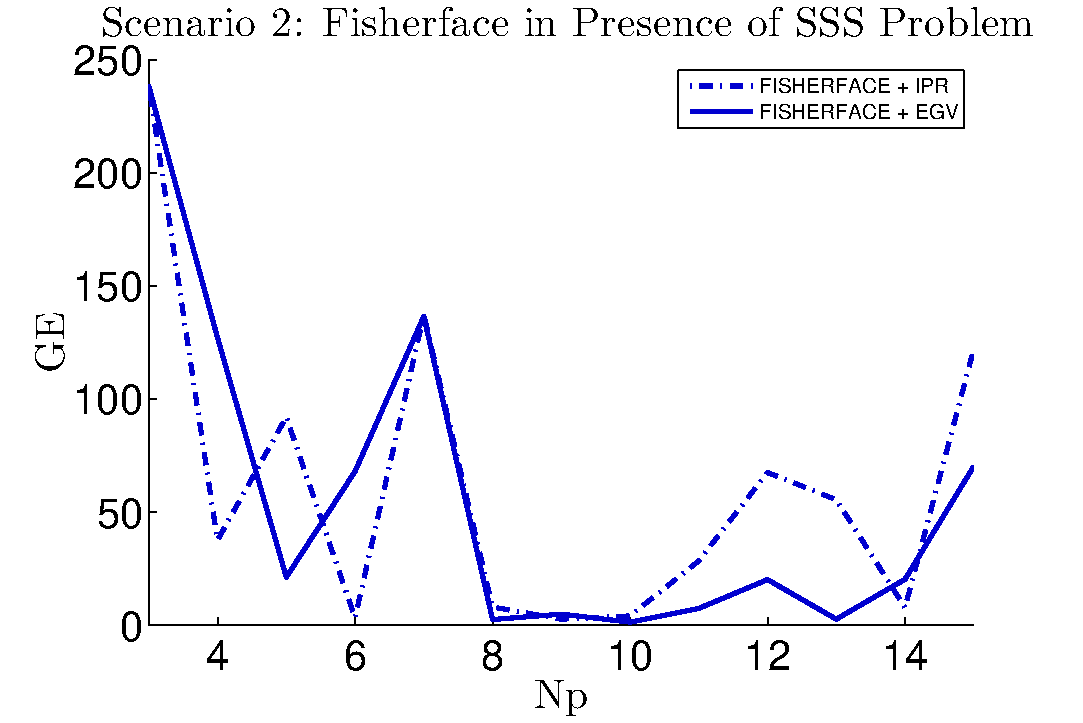
\includegraphics[width=0.5\textwidth]{../Figures/CARDIS2015/Criterion2SSS_Fisherface.pdf}}
\subfigure[]{\label{fig:direct}
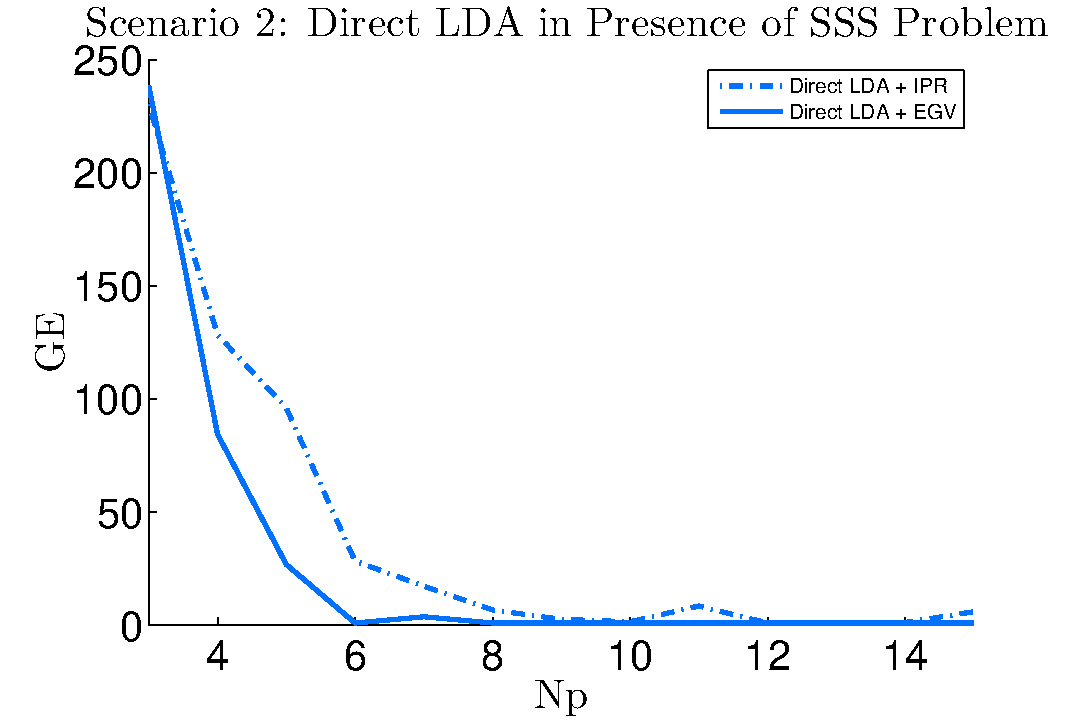
\includegraphics[width=0.5\textwidth]{../Figures/CARDIS2015/Criterion2SSS_DirectLDA.pdf}}
\subfigure[]{\label{fig:stspannedspace}
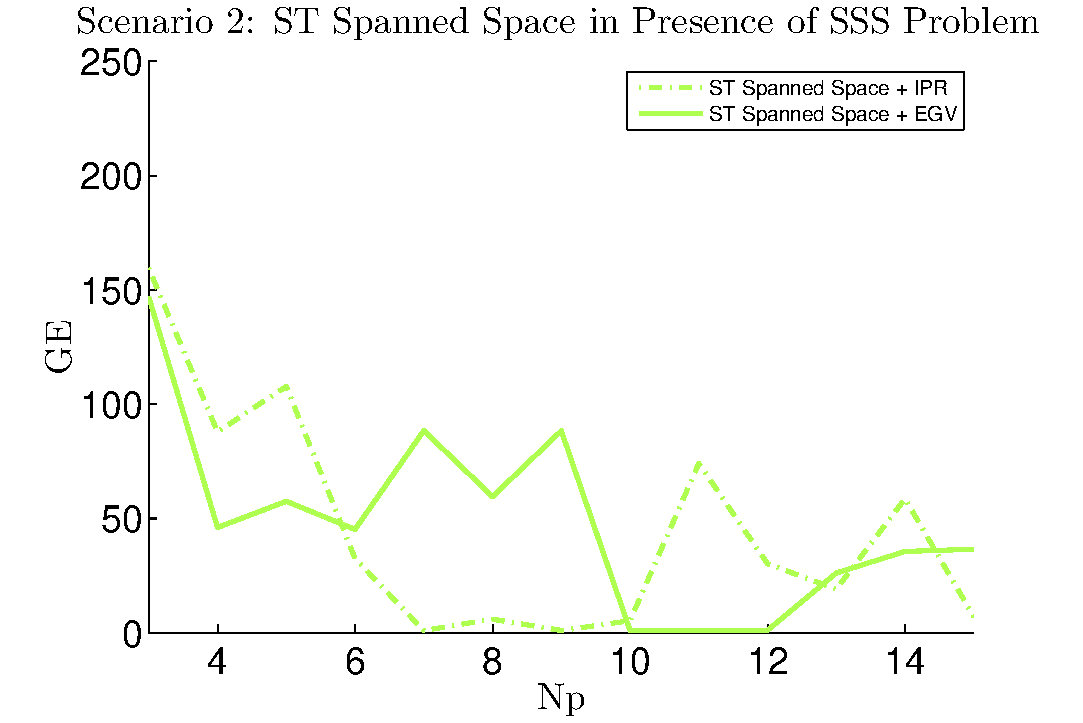
\includegraphics[width=0.5\textwidth]{../Figures/CARDIS2015/Criterion2SSS_STSpannedSpace.pdf}}
\subfigure[]{\label{fig:swnullspace}
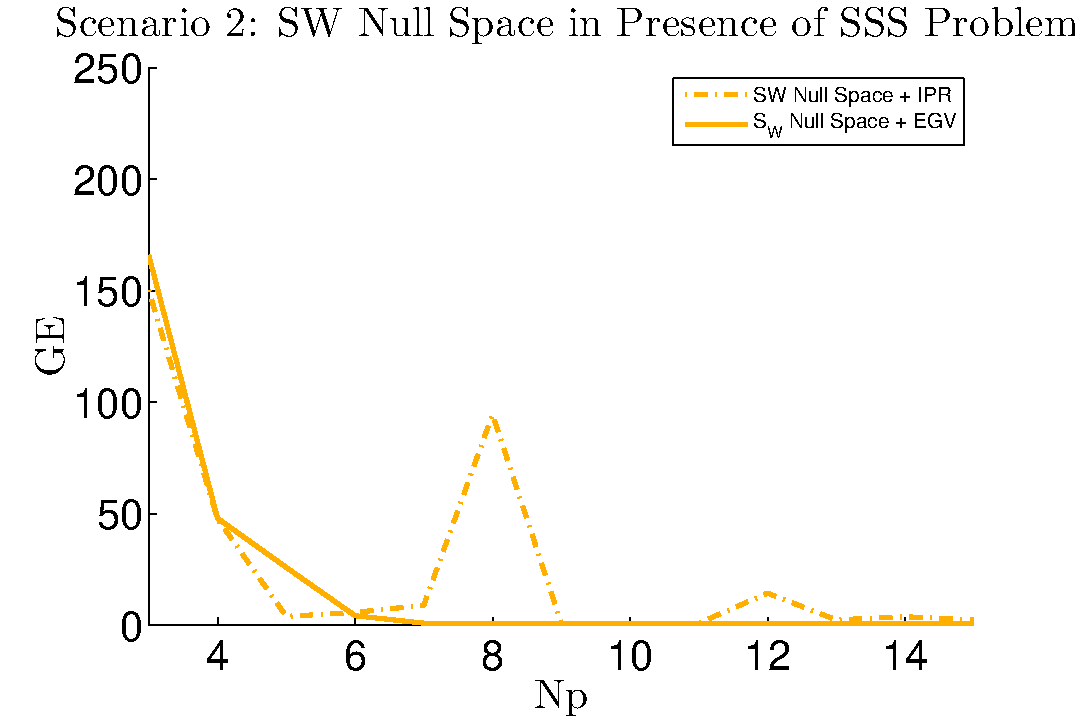
\includegraphics[width=0.5\textwidth]{../Figures/CARDIS2015/Criterion2SSS_SWnullSpace.pdf}}
\subfigure[]{\label{fig:pcaclass}
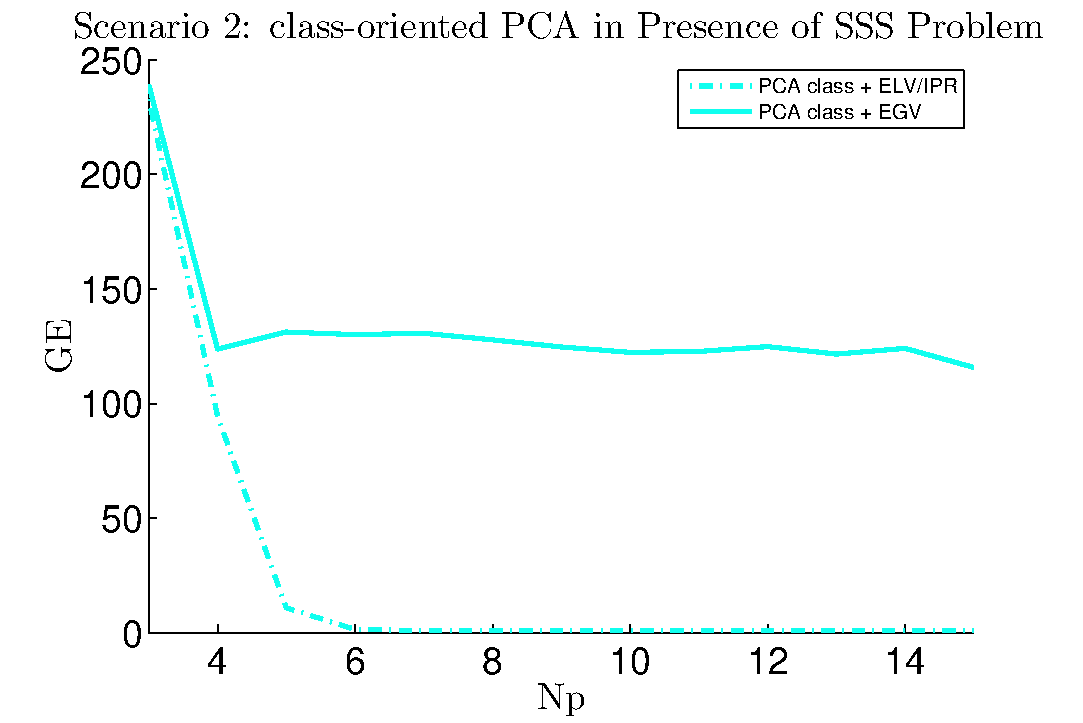
\includegraphics[width=0.5\textwidth]{../Figures/CARDIS2015/Criterion2SSS_PCAclass.pdf}}
\subfigure[]{\label{fig:notSSS}
\includegraphics[width=0.5\textwidth]{../Figures/CARDIS2015/Criterion2notSSS.pdf}}
\caption[Guessing Entropy as function of the number of profiling traces.]{Guessing Entropy as function of the number of profiling traces. Figures \subref{fig:fisherface}-\subref{fig:swnullspace}: methods extending the LDA in presence of SSS problem; Figure \subref{fig:pcaclass}: class-oriented PCA in presence of the SSS problem; Figure \subref{fig:notSSS}: number of profiling traces high enough to avoid the SSS problem.}\label{fig:scenario2}
\end{figure}

\subsection{Overview of this Study and Conclusions}
\begin{table}
\begin{tabular}{|c|c|c|c|c|c|}
\hline
&&\multicolumn{4}{|>{\columncolor[gray]{0.7}}c|}{Parameter to minimize}\\
\hline
\multicolumn{1}{|>{\columncolor[gray]{0.7}}c|}{Method}&\multicolumn{1}{|>{\columncolor[gray]{0.7}}c|}{Selection}& $N$ &  $N'$ (SSS) &  $N'$ ($\neg$SSS) &  $C$ \\
\hline
PCA standard & EGV & {\bf -} &  &{\bf -} &{\bf -} \\
\hline
PCA standard &\multicolumn{1}{|>{\columncolor[gray]{0.8}}c|}{ELV} & \multicolumn{1}{|>{\columncolor[gray]{0.9}}c|}{{\bf -}} & &\multicolumn{1}{|>{\columncolor[gray]{0.9}}c|}{{\bf -}} &\multicolumn{1}{|>{\columncolor[gray]{0.9}}c|}{{\bf -}} \\
\hline
PCA standard & IPR &{\bf -} & &{\bf -} &{\bf +} \\
\hline
PCA class & EGV & {\bf -} &{\bf -} &{\bf -} &{\bf -} \\
\hline
PCA class & \multicolumn{1}{|>{\columncolor[gray]{0.8}}c|}{ELV} &\multicolumn{1}{|>{\columncolor[gray]{0.9}}c|}{{\bf +}} &\multicolumn{1}{|>{\columncolor[gray]{0.9}}c|}{$\bigstar$}&\multicolumn{1}{|>{\columncolor[gray]{0.9}}c|}{$\bigstar$} &\multicolumn{1}{|>{\columncolor[gray]{0.9}}c|}{{\bf +}} \\
\hline 
PCA class & IPR & {\bf {\bf +}} &$\bigstar$ &{\bf +} &{\bf -} \\
\hline 
LDA & EGV &$\bigstar$ & & {\bf +} & $\bigstar$\\
\hline 
LDA & \multicolumn{1}{|>{\columncolor[gray]{0.8}}c|}{ELV} & \multicolumn{1}{|>{\columncolor[gray]{0.9}}c|}{{\bf +}} &  & \multicolumn{1}{|>{\columncolor[gray]{0.9}}c|}{{\bf +}} & \multicolumn{1}{|>{\columncolor[gray]{0.9}}c|}{$\bigstar$}\\
\hline 
LDA & IPR & {\bf +} & &{\bf +} & $\bigstar$ \\

\hline 
\multicolumn{1}{|>{\columncolor[gray]{0.8}}c|}{$\SW$ Null Space}  & EGV & &\multicolumn{1}{|>{\columncolor[gray]{0.9}}c|}{$\bigstar$ } & & \\
\hline 
\multicolumn{1}{|>{\columncolor[gray]{0.8}}c|}{$\SW$ Null Space}  & IPR & &\multicolumn{1}{|>{\columncolor[gray]{0.9}}c|}{{\bf +}} & & \\
\hline 
\multicolumn{1}{|>{\columncolor[gray]{0.8}}c|}{Direct LDA} & EGV & & \multicolumn{1}{|>{\columncolor[gray]{0.9}}c|}{$\bigstar$}& & \\
\hline 
\multicolumn{1}{|>{\columncolor[gray]{0.8}}c|}{Direct LDA} & IPR & &\multicolumn{1}{|>{\columncolor[gray]{0.9}}c|}{{\bf +}}& & \\
\hline
\multicolumn{2}{|>{\columncolor[gray]{0.8}}c|}{Fisherface} & &\multicolumn{1}{|>{\columncolor[gray]{0.9}}c|}{{\bf -}} & & \\
\hline 
\multicolumn{2}{|>{\columncolor[gray]{0.8}}c|}{$\ST$ Spanned Space}  & &\multicolumn{1}{|>{\columncolor[gray]{0.9}}c|}{{\bf -}} & & \\
\hline
\end{tabular}
\caption{Overview of extractors performances in tested situations.}\label{table:results}
\end{table}

\todo{conclusions + cita choudary choudary2018efficient che ha provato la ELV ma dice che gli ha selezionato gli stessi autovettori della EGV quindi non ha potuto osservare miglioramenti...}

%----------------------------------------------------------------------------------------
%	SECTION 7
%----------------------------------------------------------------------------------------
\section{Misaligning Effects}\label{sec:misalignment}
\todo{give parameters: 6 4}
\todo{citare Choudary, Template Attacks over different devices}
In this section we experimentally show how the approach based on linear dimensionality reduction described in this chapter is affected by traces misalignment. To this aim, we simply take the same data and parameters exploited for Scenario 1 in Sec.~\ref{sec:experiments}, and artificially misalign them through the technique proposed in Appendix~\ref{appendix:artificial_jitter} with parameters \todo{parameters here}. Then we tried to pre-process attack them through the 9 methodology tested in Scenario 1. It may be noticed in Fig.~\ref{fig:PCA_LDA_misalignment} that none of the 9 techniques is still efficient, included the optimal LDA+EGV that lead to null guessing entropy the synchronized traces using less 7 attack traces. In this case it cannot lead to successful attack in less than 3000 traces.
\begin{figure}
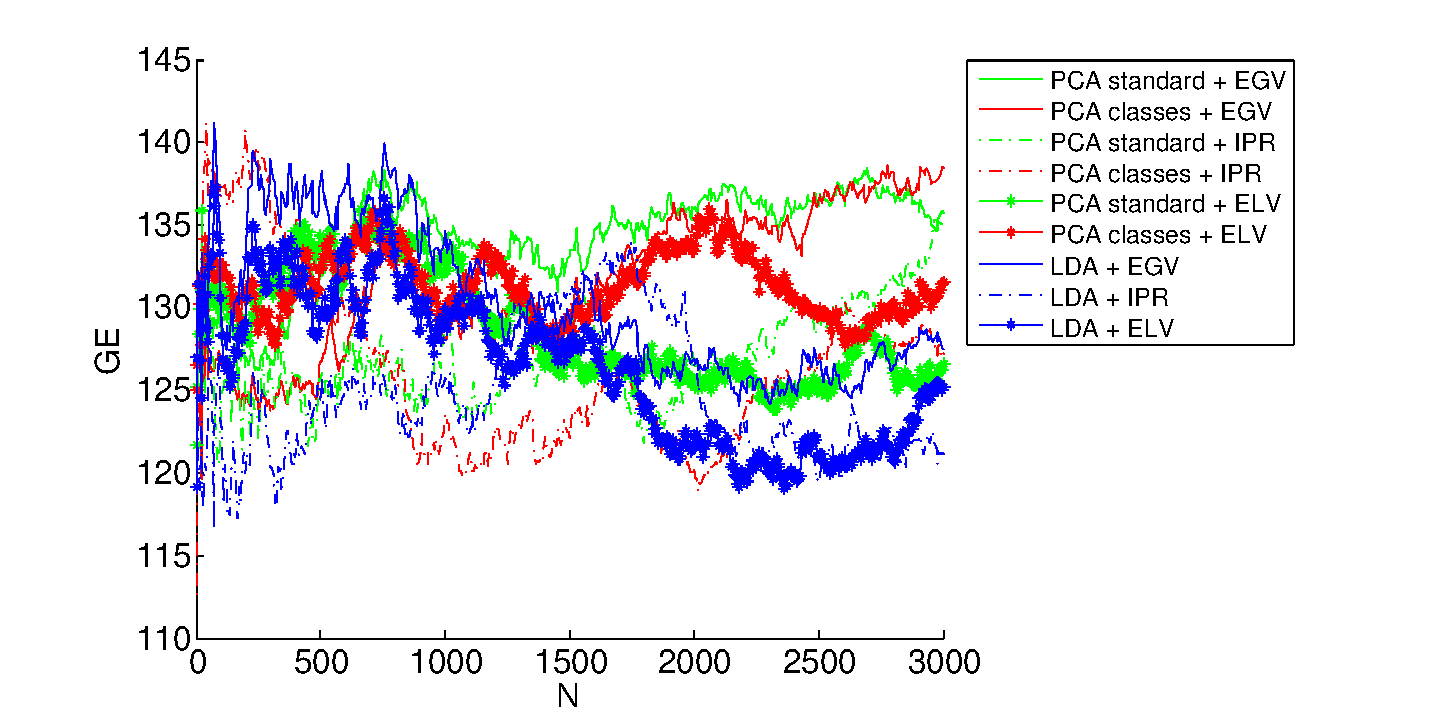
\includegraphics[width=\textwidth]{../Figures/desynchro_results_PCA_LDA.pdf} 
\caption{Degradation of linear-reduction-based template attacks in presence of misalignment.}\label{fig:PCA_LDA_misalignment}
\end{figure}